%\documentclass[a4paper,twoside,12pt]{book}
\documentclass[a4paper,twoside,12pt,openright]{book}
\usepackage[DIV=10,BCOR=3mm,headinclude=true,footinclude=false]{typearea}
%
\usepackage{booktabs}
\usepackage{jtygm}
\newcommand{\argmin}{\mathop{\rm arg~min}\limits}
\usepackage{amsmath,amssymb}
\usepackage{bm}
\usepackage[dvipdfmx]{graphicx,color,hyperref,rotating}
\usepackage{capt-of}
%\usepackage[a4paper,width=150mm,top=25mm,bottom=25mm]{geometry}
\usepackage[hang,small,bf]{caption}
\usepackage[subrefformat=parens]{subcaption}
\captionsetup{compatibility=false}
\usepackage{here}
\renewcommand{\baselinestretch}{1.2}
\hypersetup{
  colorlinks=true,
  linkcolor=blue,
  bookmarksnumbered=true,
  pdfborder={0 0 0},
  bookmarkstype=toc
}
% cref
\usepackage{cleveref}
\crefformat{section}{#2#1#3} % see manual of cleveref, section 8.2.1
\crefformat{subsection}{#2#1#3}
\crefformat{subsubsection}{#2#1#3}

%
\title{{\LARGE \sc Thesis}\\ \vspace{2zh}{\bf \LARGE A Study of Baseline Compensation System for Stable Operation of Gravitational-wave Telescope }\\ \vspace{8zh}}
\author{{\LARGE \bf Koseki Miyo} \\ \\ {\LARGE  \it Department of Physics} \\ {\LARGE \it University of Tokyo}}
\date{\vspace{1zh} \LARGE MMM 2020}
%
%
\begin{document}
\setcounter{tocdepth}{2}
\maketitle
\clearpage
\chapter*{Abstract} \addcontentsline{toc}{chapter}{Abstract}
\clearpage
%\chapter*{Abstract} \addcontentsline{toc}{chapter}{Abstract}
{\huge \bf Abstract} \\

In 2015, two LIGO detectors had directly detected the gravitational-wave (GW) from the black hole binary merger event, GW150914. In 2017, three detectors, including Virgo detector, had detected the GW from the neutron star merger, GW170817. Moreover, the electromagnetic counterpart was identified by the follow-up observations. The multi-messenger astronomy was established from this time.

GW observation needs a coincidence detection with multiple GW detectors because only a single detector cannot determine the direction of the GW source. If multiple detectors detect the GW, we can estimate the direction from the differences of these detection times. In order to determine the direction, at least three GW detectors are needed. However, the duty cycle of the GW detectors is almost 60 \%, and the duty cycle of the multiple detectors is below 50\%. 

This duty cycle is limited by the unstable operation of GW detectors, which is caused by the seismic disturbance mainly below 1 Hz. While these seismic noises disturb the baseline in this frequency, the current vibration isolation system for GW detectors does not have the isolation performance in this low-frequency seismic noise, because of the insufficient sensitivity of the inertial sensor used in this isolation system. 

In this study, the baseline compensation system has been developed. Unlike the current vibration isolation system, this system uses a 1500 m strainmeter installed in parallel KAGRA baseline, which is named geophysics interferometer (GIF). GIF is designed and developed for monitoring the deformation of the baseline directly below 1 Hz with high sensitivity. For this reason, we designed the new system to compensate for the baseline so that KAGRA interferometer would not be affected by low-frequency seismic disturbances.

In this thesis, two main topics are described: the influence of the seismic disturbances to GW detectors and the baseline compensation system to attenuate these disturbances. The design, the performance, and the advantage of this new system are described. Moreover, the implementation and demonstration of this system on KAGRA interferometer are also described. In the test demonstration, the baseline compensation system is installed on the X-arm cavity, which is the most sensitive component in the GW detectors. As a result, the cavity length fluctuation caused by the deformation of the baseline is reduced by -6 dB above 0.01 Hz and by -20 dB below this frequency.

This result would increase the duty cycle of KAGRA interferometer. If this new vibration isolation system can be installed in other GW detectors, the coincidence duty cycle can also be improved. 

\clearpage
\chapter*{要旨} \addcontentsline{toc}{chapter}{要旨}
%\clearpage
%\chapter*{要旨} \addcontentsline{toc}{chapter}{要旨}
%{\huge \bf 要旨} \\

2015年、LIGO の2台の重力波検出器がブラックホール連星合体イベントからの重力波 GW150914 を直接検出することに成功した。2年後の2017年には Virgo を加えた3台の重力波検出器で連星中性子合体イベントからの重力波 GW170817 を検出した。この重力波イベント直後のフォローアップ観測によって電磁波対応天体も同定され、これによりマルチメッセンジャー観測が確立された。

重力波観測には本質的に3台以上の検出器での同時観測が必要である。なぜならば単体検出器だけでは到来方向が定まらないためである。複数台で重力波を検出すれば、それらの到来時間差から到来方向が定まる。十分な到来方向を得るためには、最低でも3台の検出器で重力波を観測しなければならない。このように同時観測が必須な重力波検出器であるが、GW170817 を観測した第二次観測期間(O2)での、単独検出器の duty cycle は $60\,\%$ 程度であった。複数台の duty cycle は半分も満たない。

この duty cycle 低下の最大の原因は、おもに 1 Hz 以下の低周波地面振動である。

重力波検出器は鏡の変位測定に対して高感度であるが故に非常に狭い範囲でしか動作しない。現在の重力波検出器は、腕に km スケールの Fabry-Perot 光共振器をもつ Michelson 干渉計である。この干渉計の感度を維持させるには腕共振器を共振状態に保たなければならず、それはつまり、腕共振器長を数 nm の線幅以下に防振しなければならないことを意味する。したがって腕共振器鏡は振り子をつかって防振される。振り子をつかった受動防振は、多段にして防振比を高め、低共振周波数にしてより低周波の地面振動を防振することができる。しかし実際の振り子の共振周波数はせいぜい 1 Hz 弱であり、それ以下の地面振動は防振することができない。これに対して脈動と呼ばれる地面振動が$200\,\mathrm{Hz}$ 付近で地面を揺らす。この地面振動は波浪が海底を叩くことで生じ、その振幅は天候に強く左右され、悪天候時では数 um におよぶ。これは腕共振器の線幅よりもはるかに大きく、duty cycle の低下を直接意味する。このように、振り子を用いた受動的な防振だけでは低周波地面振動を防振することは困難である。

そこで、能動防振と呼ばれるアイデアが生まれた。このアイデアは、振り子の懸架点を支えるステージの動きをセンサーで測定し、それを打ち消すように能動的にステージを動かして防振するというものである。この制御で使われるセンサーには2つの種類がある。一つは地震計である。この地震計はステージの上に置かれ、その出力信号が小さくなるように ステージが feedback 制御され防振される。地震計はその原理から慣性センサーともよばれ、慣性系からみた地面振動を測定する。つまり地震計を用いた能動防振はステージを慣性系に対して防振することを意味する。しかし一般に地震計は低周波では感度が悪く、また tilt-holizontal coupling と呼ばれる、並進方向の地面振動が地震計の傾斜と区別がつかない信号カップリングがあり、およそ $100\,\mathrm{Hz}$ 以下では制御に使うことができない。一方でこれに対してもう一つは、suspension point interferometer (SPI) と呼ばれる干渉計である。SPIは腕共振器鏡を防振する振り子の懸架点間の距離を直接測ることができる。これを用いた能動防振は、地震計をつかった能動防振のように低周波で性能を制限されることがない。このような利点をもつSPIだが、km スケールの重力波検出器で SPI を構築する場合、SPI自身を干渉させるための角度制御が必要になるなどの技術的な困難が多く、実際の能動防振には地震計方式が用いられている。しかしやはりこの方式では、脈動は防振することができるが、100 Hz 以下の地面振動は防振できないままである。とくに、100 mHz から数 10 $\mathrm{mHz}$までの帯域では、比較的規模の大きい地震が地面を励起する。このような規模が大きい地震の場合、揺れの継続時間は数時間にもおよぶ。実際、マグニチュード6以上の地震が原因で干渉計が動作できないロックロス状態を引き起こすことが報告されており、O2での duty cycle はこの揺れによって制限されていた。

本研究では、geophysics interferometer (GIF) と呼ばれる 1.5 km のレーザーひずみ計を、 SPI として用いる能動防振の開発をおこなった。このGIF は、2つある KAGRA の 3 km の腕のうち、片腕の X アームに併設されている。このひずみ計は、地震研究所が地殻変動を精密に計測するために開発したものであり、地殻変動を直接測るために、その鏡は岩盤に固定されている。また鏡にはコーナーキューブを使用しているため、 km スケールの角度制御を必要としない。GIFは非常に安定して稼働しており、稼働を開始した2016年秋からおよそ3年間地殻変動の観測をおこなっている。このように基線長変動を測定できる GIF の信号をつかって、腕共振器を懸架するステージを feedforward 制御し、基線長が一定になるように防振をする基線長補償システムを構築した。

本論文では、地面振動が重力波検出器に与える影響について調べられており、そしてその影響を低減するための基線長補償システムの原理と、その理論的性能、既存のシステムと比較した利点が述べられている。また、このシステムを実際のKAGRAに組み込んだ性能評価実験が述べられている。この実験では、 GIF の信号をつかって Xアームの 3 km Fabry-Perot 光共振器長を防振した際の腕共振器長変動を測定した。その結果、腕共振器長の残留振動は、 0.01 Hz 以上では半分に、それ以下の帯域では約10分の1に抑えられた。

この結果から、基線長補償システムは KAGRA の duty cycle を向上させることが期待される。また、この手法は他のLIGOとVirgoにも適用可能であり、適用された場合、同時観測の duty cycle も向上が期待される。

\clearpage
\tableofcontents
%\listoffigures
%% \chapter{Background}
\section{Gravitational-wave}
\subsection{...}
\section{Sources of gravitational-wave}
\subsection{...}
\section{Interferometric Gravitational-wave detection} \label{sec:13}
\subsection{Introduction}
\subsection{Detection Principle}
\subsection{The 2nd Generation Interferometers}
\subsection{Working Principle}
\subsubsection{Fabry-Perot Cavity}
\subsubsection{Power Recycling Cavity}
\subsubsection{Signal Recycling Cavity}
\section{Summary of the Chapter}
 % Background
%% \chapter{Seismic Noise}
Seismic noise causes two issues for laser interferometric gravitational-wave detectors; (1) limitation of the low-frequency sensitivity of the detectors and (2) deterioration of the duty cycle of that. The seismic noise above $1\,\mathrm{Hz}$, which is associated with anthropogenic activity, contaminates the low-frequency sensitivity. The seismic motion below this frequency, which is generated by the natural noise source such as the ocean, disturbe the Fabry-Perot arm cavity to resonate stably.

In order to resolve these issues, a laser interferometer gravitational wave antenna with a baseline length of 20 m (LISM) \cite{sato2004ultrastable} is constructed underground, because the low-level seismic noise is expected in the undeground environment. As a result, the seismic noise in LISM site is less than that in the surface site by two prders of magnitude in $1$--$100\mathrm{Hz}$ region, and the underground GW detector performanced stable operation with duty cycle of $99.8 \%$.

However, for km-meter scale GW detector like KAGRA, such a stable operation can not be expected because
\begin{itemize}
  \setlength{\itemsep}{1pt}      %2. ブロック間の余白
  \setlength{\parskip}{-1pt}     %4. 段落間余白.
  \setlength{\itemindent}{0pt}   %5. 最初のインデント
  \setlength{\labelsep}{5pt}     %6. item と文字の間
\item length of the long baseline is susceptible to the low-frequency seismic motion compared with the short one due to the a few reduction effect kind of the {\it common mode rejection}, and this problem is common in not only all the current detectors but also the next $10\,\mathrm{km}$-scale detectors; Einstein Telescope (ET)\cite{punturo2010einstein} and Cosmic Exploler (CE) \cite{abbott2017exploring}.
\item especially in KAGRA site, the microseismic noise corelated with the ocean activity in $0.03$--$0.3\,\mathrm{Hz}$, which is the most problematic noise for stable operation of GW detector, cannot be reduced even in the underground due to near the sea ($40\,\mathrm{km}$ from Toyama Bay), and this problem is common in ET which is also will be constructed in underground but in island \cite{naticchioni2014microseismic}.
\end{itemize}
The purpose of this chapter is to describe quantitatively above two problems. In this chapter, first, section \cref{sec:31} gives an theoretical understanding of the seismic noise as the elastic waves. In section \cref{sec:32}, some general properties of the seismic noise are described by quotting previous researches. Finally, we discuss the problems in section \cref{sec:33}.



\section{Theory of seismic waves} \label{sec:31}
Here we introduce characteristics of the seismic wave that will be usefull in our later understanding and modeling of seismic effects.



\subsection{Seismic Waves}
The elastrodynamic wave equation without external forces is given by 
\begin{eqnarray}\label{eq:eq_1}
  \rho{\bm{\ddot{u}}} = (\lambda+2\mu)\nabla(\nabla\cdot\bm{u}) - \mu\nabla\times(\nabla\times\bm{u}),
\end{eqnarray}
where $\bm{u}$ is the displacement field vetor of the medium, $\rho$ denotes density of the medium, and $\lambda,\,\mu$ are Lame's first and second parameter.



\subsubsection{Body Waves}
From Eq.(\ref{eq:eq_1}), we can obtain two characteristic waves; longitudinal wave (primary wave, P-wave) and transverse wave (secondary wave, S-wave). First, using Helmholtz's decomposition, we represent the displacement field vector $\bm{u}$ as
\begin{eqnarray} 
  \bm{u} &=& \nabla\phi + \nabla\times\bm{\psi}, \label{eq:eq_4}
\end{eqnarray}
where $\phi$ the scalar potential and $\bm{\psi}$ are the vector potential. Each term of Eq.(\ref{eq:eq_4}) show the divergent and the rotation component of $\bm{u}$ respectively. Substitute Eq.(\ref{eq:eq_4}) into Eq.(\ref{eq:eq_1}) and after some vector algebra, one can obtain two wave equations;
\begin{eqnarray}
  \ddot{\phi} &=& v_{L}^2\nabla^2\phi \label{eq:eq_5},\\
  \ddot{\psi} &=& v_{T}^2\nabla^2\psi \label{eq:eq_6}, 
\end{eqnarray}
where $v_{L},\,v_{T}$ are defined as 
\begin{eqnarray}
  v_{L} = \sqrt{\frac{\lambda+2\mu}{\rho}},\
  v_{T} = \sqrt{\frac{\mu}{\rho}}. \label{eq:eq_7}
\end{eqnarray} 
These phase velocities; $v_{L},v_{T}$ represent that of the P-wave and the S-wave. Show this relationships. Because the scalar potential and the vector potential are obey the wave equation Eq.(\ref{eq:eq_5}) and Eq.(\ref{eq:eq_6}) respectivly, the general solutions of these potentials are given as
\begin{eqnarray}
  \phi &=& \phi_{0}(\omega{t}-\bm{k}\cdot{\bm{x}}) \label{eq:eq_8}\\
  \bm{\psi} &=& \bm{\psi_{0}}(\omega{t}-\bm{k}\cdot{\bm{x}}) \label{eq:eq_9},
\end{eqnarray}
where $\omega,\,\bm{k}$ are the angler frequency and the wave vector. One can obtain the divergent component of displacement filed vector $\bm{u}$ as
\begin{eqnarray}
  \bm{u}_{\mathrm{div}} = \nabla{\phi_{0}(\omega{t}-\bm{k}\cdot{\bm{x}})} =-\bm{k}{\phi}.
\end{eqnarray}
The displacement of this wave $\bm{u}_{\mathrm{div}}$ whose phase velocity is $v_{L}$ propagates along with direction of the wave vector. Therefore $v_{L}$ is the phase velocity of a longitudinal wave called P-wave. On the other hands, one can obtain the rotation component of $\bm{u}$ as
\begin{eqnarray}
  \bm{u}_{\mathrm{rot}} = \nabla\times{\bm{\psi_{0}}(\omega{t}-\bm{k}\cdot{\bm{x}})} =-\bm{k}\times{\bm{\psi}}.
\end{eqnarray}
This displacement vector $\bm{u}_{\mathrm{rot}}$ whose phase velocity is $v_{T}$ is perpendicular to the wave vector. Therefore, $v_{T}$ is the phase velocity of a transverse wave called S-wave. Furthermore, because  $\lambda$ and $\mu$ are positive numbers, 
\begin{eqnarray}
  v_{L} > v_{T}.\label{eq:eq_10}
\end{eqnarray}
Therefore, the longituginal wave is faster than the transverse wave.



\subsubsection{Rayleigh waves}
\textcolor{red}{
  Rayleigh wave はP波とS波の干渉によって生じる\cite{}。ここではZ軸を鉛直方向とした直交直線座標系のx-z面内で振動する弾性波を考える。z=0を自由表面とし、x軸に沿ってP波とS波が同じ速度$v_{R}=\omega/k$ ($\omega$ is anglar frequency and $k$ is the wave vector) で伝搬する場合を考えると、ポテンシャル$\phi$と$\bm{\psi}$は、それぞれ以下のように表すことができる。
\begin{eqnarray}
  \phi &=& F(z)\exp[i(kx-\omega{t})],\label{eq:eq_12}\\
  \psi &=& G(z)\exp[i(kx-\omega{t})]\label{eq:eq_13}
\end{eqnarray}
Eq.\ref{eq:eq_12}とEq.\ref{eq:eq_12}を波動方程式Eq.\ref{eq:eq_5},Eq.\ref{eq:eq_6}に代入すれば、レイリー波の特性方程式が導かれる;
\begin{eqnarray}\label{eq:eq_11}
\left(\frac{c_{R}^{2}}{c_{S}^{2}}\right)^{3}-8\left(\frac{c_{R}^{2}}{c_{S}^{2}}\right)^{2}+8\left(3-\frac{2}{\gamma^2}\right)\left(\frac{c_{R}^{2}}{c_{S}^{2}}\right)-16\left(1-\frac{1}{\gamma^2}\right)=0
\end{eqnarray}
where $\gamma\equiv v_{L}/v_{T}$. In case that $0 < (\frac{c_{R}^2}{c_{S}^2}) <1$, the velocity has physically meaningful value. According to Eq.\ref{eq:eq_11}, the ratio $\frac{c_R}{c_S}$ is a function of the ratio of $\gamma$. たとえば、KAGRAと同じ山の下に建設された100mの重力波望遠鏡CLIOでのP波とS波の位相速度はそれぞれAA、BBである\cite{takemoto2003}ので、$\gamma = 1.82 $である。したがってこのときのレイリー波の位相速度はCCである。
}



\subsection{Reduction Effect in the Deep Sites}
\textcolor{red}{
  レイリー波の振幅は深さに依存しており、深いほど小さくなる。
}



\subsection{Reduction Effect of the Short Baseline} \label{sec:313}
For interferometric gravitational-wave detectors which need a precise length control of the optical resonate cavity, it is appropriate to consider about the relative displacement between two points rather than the displacement of single point.



\subsubsection{Differential Motion and Common Motion}
We define the motion of two points shown in Fig.(\ref{img:img310}) as $\bm{u}_1=\bm{u}(t,\bm{x}_1)$ and $\bm{u}_2=\bm{u}(t,\bm{x}_2)$, respectively. The motions of the two points can be represented as the differential motion and the common motion. The displacement of both differential motion and common motion of the two points shown in Fig.(\ref{img:img310}) are defined as
\begin{eqnarray}
  \bm{u}_{\mathrm{diff}} \equiv \frac{\bm{u}_{1}-\bm{u}_{2}}{\sqrt{2}}, \, \\ \label{eq:eq22}
  \bm{u}_{\mathrm{comm}}  \equiv \frac{\bm{u}_{1}+\bm{u}_{2}}{\sqrt{2}} \label{eq:eq100}
\end{eqnarray}
These two motions defined in Eq.(\ref{eq:eq22}) and Eq.(\ref{eq:eq100}) are normalized by $\sqrt{2}$ to conserve the total power.
\begin{figure}[h]
  \begin{center}
    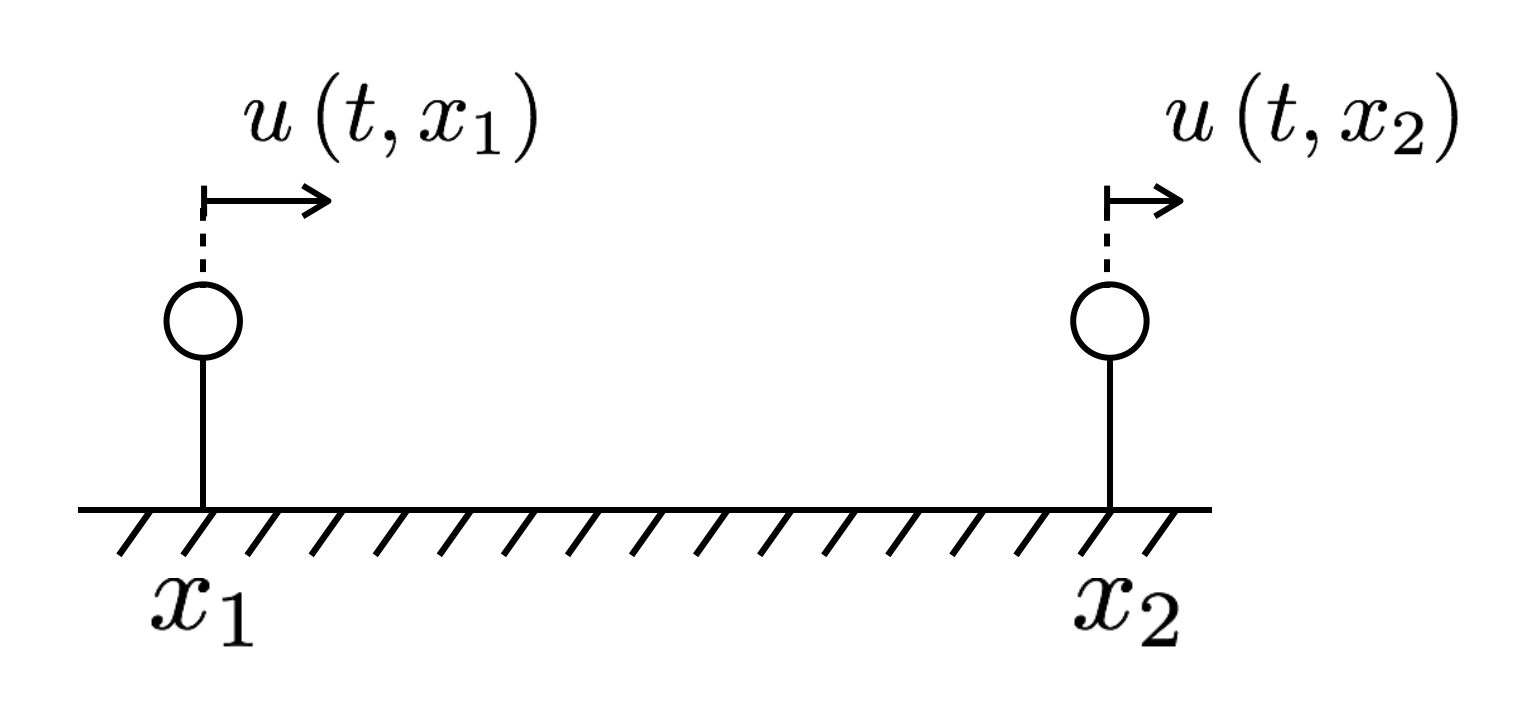
\includegraphics[width=9.0cm]{./img_chap3/img315.png}
    \caption{The displacements of the two points which are sparated L in X axis. $\bm{u}(t,\bm{x})$ is the displacement field vector, where $t$ denotes the time and $\bm{x}$ denotes the location vector.}\label{img:img310}    
  \end{center}
\end{figure}



\subsubsection{Common and Differential Motion Ratio (CDMR)}\label{sec:sec313}
We define the power ratio of the common motion over the differential motion as common and differential motion ratio (CDMR). This ratio is usefull to describe how the differential motion is reduced in the baseline compared to the common motion. CDMR is defined as
\begin{equation}
  \mathrm{CDMR} \equiv \sqrt{\frac{\mathrm{Common\,Motion}}{\mathrm{Differential\,Motion}}} = \sqrt{\frac{P_{\mathrm{comm}}(\omega)}{P_{\mathrm{diff}}(\omega)}} \label{eq:eq23}
\end{equation}
where $P_{\mathrm{comm}},P_{\mathrm{diff}}$ are the power spectral densities (PSDs) of the differential motion and common motion, respectively. In order to obtain these PSDs, we convert from the autocorrelation function of these. Therefore, first, autocorrelation function $C_{\mathrm{diff}}$ of the differential motion is given by its definition in Eq.(\ref{eq:eq22})
\begin{eqnarray}
  C_{\mathrm{diff}}(\tau) &=& \frac{1}{2}
  \biggl\langle
  \biggl[ x_{1}(t)-x_{2}(t) \biggr] \biggl[ x_{1}(t+\tau)-x_{2}(t+\tau) \biggr]
  \biggr\rangle \\
  &=& \frac{1}{2}\biggl[ C_{11}(\tau) - C_{12}(\tau) - C_{21}(\tau) + C_{22}(\tau) \biggr], 
\end{eqnarray}
,where $C_{ij}$ are the autocorrelation functions of each point and defined as $ C_{ij} \equiv \langle x_{i}(t)x_{j}(t+\tau)\rangle,\, (i=1,2,\,j=1,2)$. Here, one can obtain the power spectrum density of differential motion $P_{\mathrm{diff}}(\omega)$ as 
\begin{eqnarray}
  P_{\mathrm{diff}}(\omega) &=& \frac{1}{2}\biggl[ P_{1}(\omega) + P_{2}(\omega) - P_{12}(\omega) - P_{12}^*(\omega) \biggr]\\
  &=& \frac{1}{2} \biggl[ P_{1}+P_{2} - \mathrm{Re}\left[\gamma \right]\times2\sqrt{P_{1}P_{2}} \biggr], \label{eq:eq31}
\end{eqnarray}
where $P_{1}(\omega),P_{2}(\omega)$ are the power spectrum densities of each points, and $P_{12}(\omega)$ are the cross spectrum between two point. The parameter $\gamma$ is the complex coherence between them defined by
\begin{eqnarray}
  \gamma \equiv \frac{P_{12}}{\sqrt{P_{1}P_{2}}}.
\end{eqnarray}
Furthermore, assuming that seismic wave propagating each points does not decay, which means $P_{1}=P_{2} \equiv P$, one can compute the $P_{\mathrm{diff}}(\omega)$ as 
\begin{eqnarray} \label{eq:eq32}
  P_{\mathrm{diff}}(\omega) = P (1-\mathrm{Re}\left[\gamma\right]).
\end{eqnarray}
Similarly, the PSD of the common motion can be calculated as
\begin{eqnarray}
  P_{\mathrm{comm}}(\omega) = P (1+\mathrm{Re}\left[\gamma\right]).
\end{eqnarray}
Finaly, CDMR defined Eq.(\ref{eq:eq23}) in case the seismic wave does not decay is represented as
\begin{eqnarray}
 \mathrm{CDMR} = \sqrt{\frac{1 + \mathrm{Re} \left[\gamma \right] }{1 - \mathrm{Re} \left[\gamma \right]}}\,. \label{eq:eq33}
\end{eqnarray}
Eq.(\ref{eq:eq33}) indicates that CDMR can be expressed by only the coherence $\gamma$ between of two points. For example, CDMR tends to be larger when $\gamma$ close to 1. This means that the differential motion is more less than the common motion because the two points move together in the same direction.



\subsubsection{Uniform Plane Wave Model}
Consider the CDMR when the plane waves are distributed uniformly around the azimuth. Because the coherence that the single plane wave propagating with the azimuth angle $\theta$ along the direction of arm cavity from $x_1$ to $x_2$ in Fig.(\ref{img:img310}) is 
\begin{equation}
  \gamma = e^{i\frac{L\mathrm{cos}\theta\omega}{c}}, \label{eq:eq18}
\end{equation} 
the coherence in case that the plane waves propagats uniformly is given by the integral of Eq.(\ref{eq:eq18}) over all direction;
\begin{eqnarray} \label{eq:eq19}
  \gamma &=& \frac{1}{2\pi} \int_{-\pi}^{\pi} e^{i\frac{\omega}{c} L\cos \theta} d \theta .
\end{eqnarray}
where the coherence is normized azimuth angle. Therefore, the CDMR is given as
\begin{equation}  \label{eq:eq20}
  \mathrm{CDMR} = \sqrt{\frac{1+J_0(\frac{L\omega}{c})}{1-J_0(\frac{L\omega}{c})}} .
\end{equation}

For later discussion in \cref{sec:332}, the PSD of the differential motion in case of the uniform seismic waves is usefull and is given as
\begin{eqnarray} \label{eq:eq21}
  P_{\mathrm{diff}}(\omega) = P \left[1-J_0\left(\frac{L\omega}{c}\right)\right] .
\end{eqnarray}

\begin{figure}[p]
  \begin{center}
    \centering
    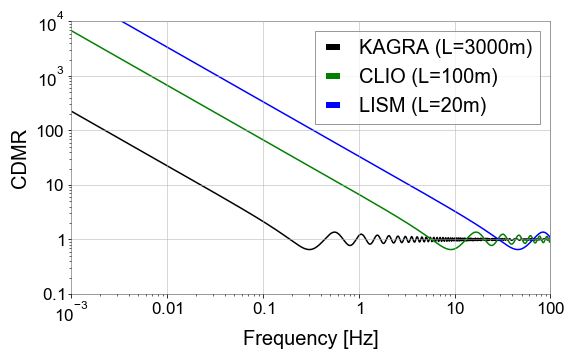
\includegraphics[width=12cm]{./img_chap3/img329.png}
    \caption[CDMR, which is the power ratio of the common motion over the differential motion of baseline in Eq.(\ref{eq:eq20}), of the underground GW detectors assuming the uniform plane waves model with phase velocity of 3000 m/sec.]{CDMR, which is the power ratio of the common motion over the differential motion of baseline in Eq.(\ref{eq:eq20}), of the underground GW detectors assuming the uniform plane waves model with phase velocity of 3000 m/sec. Black is KAGRA with the 3000 m baseline, green is CLIO with the 100 m baseline, and blue is LISM with the 20 m baseline. The CDMR of the long baseline is worse than that of short baseline. For example, at $0.1\,\mathrm{Hz}$, if the baseline length is longer, the CDMR is larger..}\label{img:img301}
    \centering      
    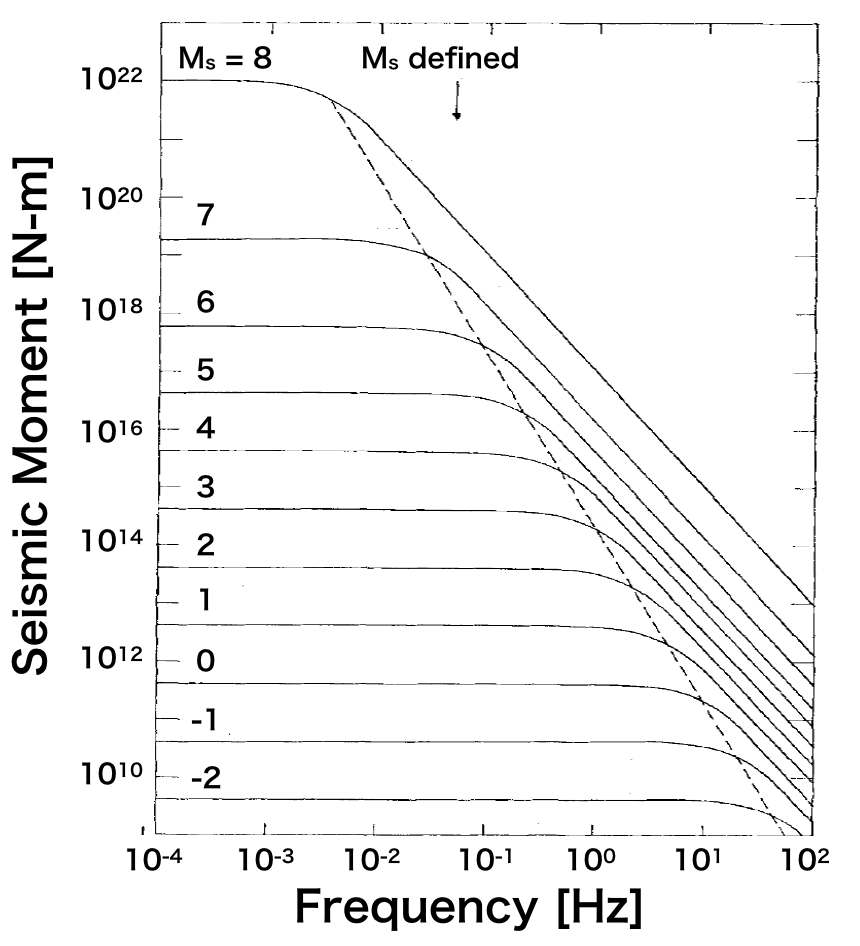
\includegraphics[width=12cm]{./img_chap3/img328.png}
    \caption[The power ratio of the differential motion of the baseline over the motion at single point; $P_{\mathrm{diff}}/P$ of Eq.(\ref{eq:eq21})]{The power ratio of the differential motion of the baseline over the motion at single point; $P_{\mathrm{diff}}/P$ of Eq.(\ref{eq:eq21}). This ratio gives the estimation of the PSD of baseline length fluctuation from the }\label{img:img302}
  \end{center}
\end{figure}



\section{Seismic Noise}\label{sec:32}
Here we describe the actual seismic noise. Characteristics of the seismic noise are related with its origin spatially and temporally. The noise sources are spreaded anywhere; foot steps, traffics and ocean waves, and these amplitude depends on day-night or weather condition.

As summarized in Table \ref{tb:31}, the seismic noises above $1\,\mathrm{Hz}$ are cleary correlated with cultural activities, and that below this frequency are excited by the natural phenomena \cite{bonnefoy2006nature}.
\begin{table}[h] 
  \begin{center}
    \caption{Two types of seismic noise}\label{tb:31}
    \begin{tabular}{lll} 
      \hline      
      Type of noise & Frequency Band & Sources \\ \hline \hline
      Cultural Noise & $> 1\,\mathrm{Hz}$ & wind, traffic, machinaries, foot steps\\
      Natural Noise  & $< 1\,\mathrm{Hz}$ & ocean, air pressure, earth tides\\
    \end{tabular}
  \end{center}
\end{table}

This boundary frequency between cultural or natural is depends on the soil structure. At the sediment site such as the LIGO\cite{Daw_2004} and Virgo site\cite{Beker_2012}, the cultural noise can be shifted to a lower frequency and appear below $1\,\mathrm{Hz}$. On the other hands, at the hard rock site such as KAGRA site, the cultural noise can be distinguished from the natural noise for its diurnal variability and apparent only above $1\,\mathrm{Hz}$.


\subsection{Cultural Noises} \label{sec:321}
The cultural seismic noise contaminates the sensitivity of gravitational-wave detectors in the frequency range of interest for gravitational-waves sources, above $1\,\mathrm{Hz}$. In this frequency band, the cultural noise is dominated by winds or human activities. For example, seismic noise from traffic near the detectors is reported at LIGO site \cite{schofield2000source}, and noise from the vibrations of building excited by winds is reported at Virgo site \cite{acernese2004properties}. 

\subsection{Natural Noises} \label{sec:322}
The natural seismic noise affects the stability of the GW detectors below $1\,\mathrm{Hz}$ because it deforms largely the ground on which mounted the detectors.

これらnatural seismic noise は場所によって大きくことなることが知られている。Petersonらによって行われた、世界の75箇所の基地にある地震計の数年分のデータから得た地面振動のノイズスペクトルをFigure \ref{img:img324}に黒線で示す。$200\,\mathrm{mHz}$のピークは

\begin{figure}[p]
  \begin{center}   
    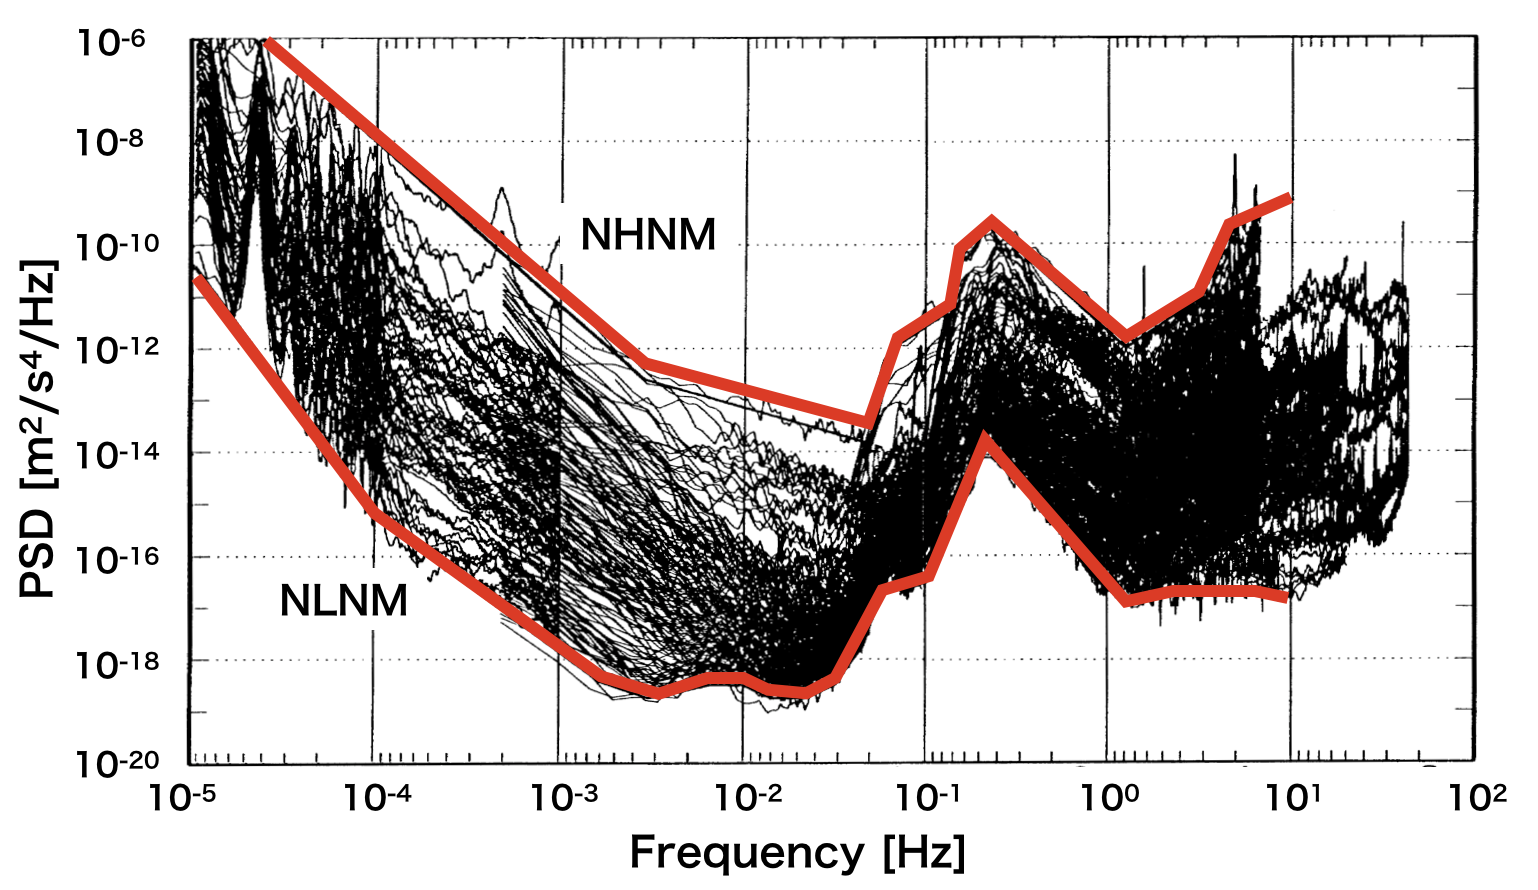
\includegraphics[width=12.5cm]{./img_chap3/img324.png}
    \caption{PSDs of the seismic noise obtained by Peterson in 75 stations in the world \cite{peterson1993observations}. Each of the black solid lines is PSD divided into 5 different frequency band at the each stations. Each red lines are the new high noise model (NHNM) and the new low noise model (NLNM), respectively. The NHNM a spectrum of average high background noise power in the seismometer network, and the primary contributions to NHNM are inland stations situated on soft solid in very noisy locations and coastal stations with high amplitude microseisms. The NLNM represents the seismic noise when microseismic is quiet, and below microseismic, it represents the global seismic noise floor\cite{nishida2002origin}.}\label{img:img324}
  \end{center}
  \begin{center}   
    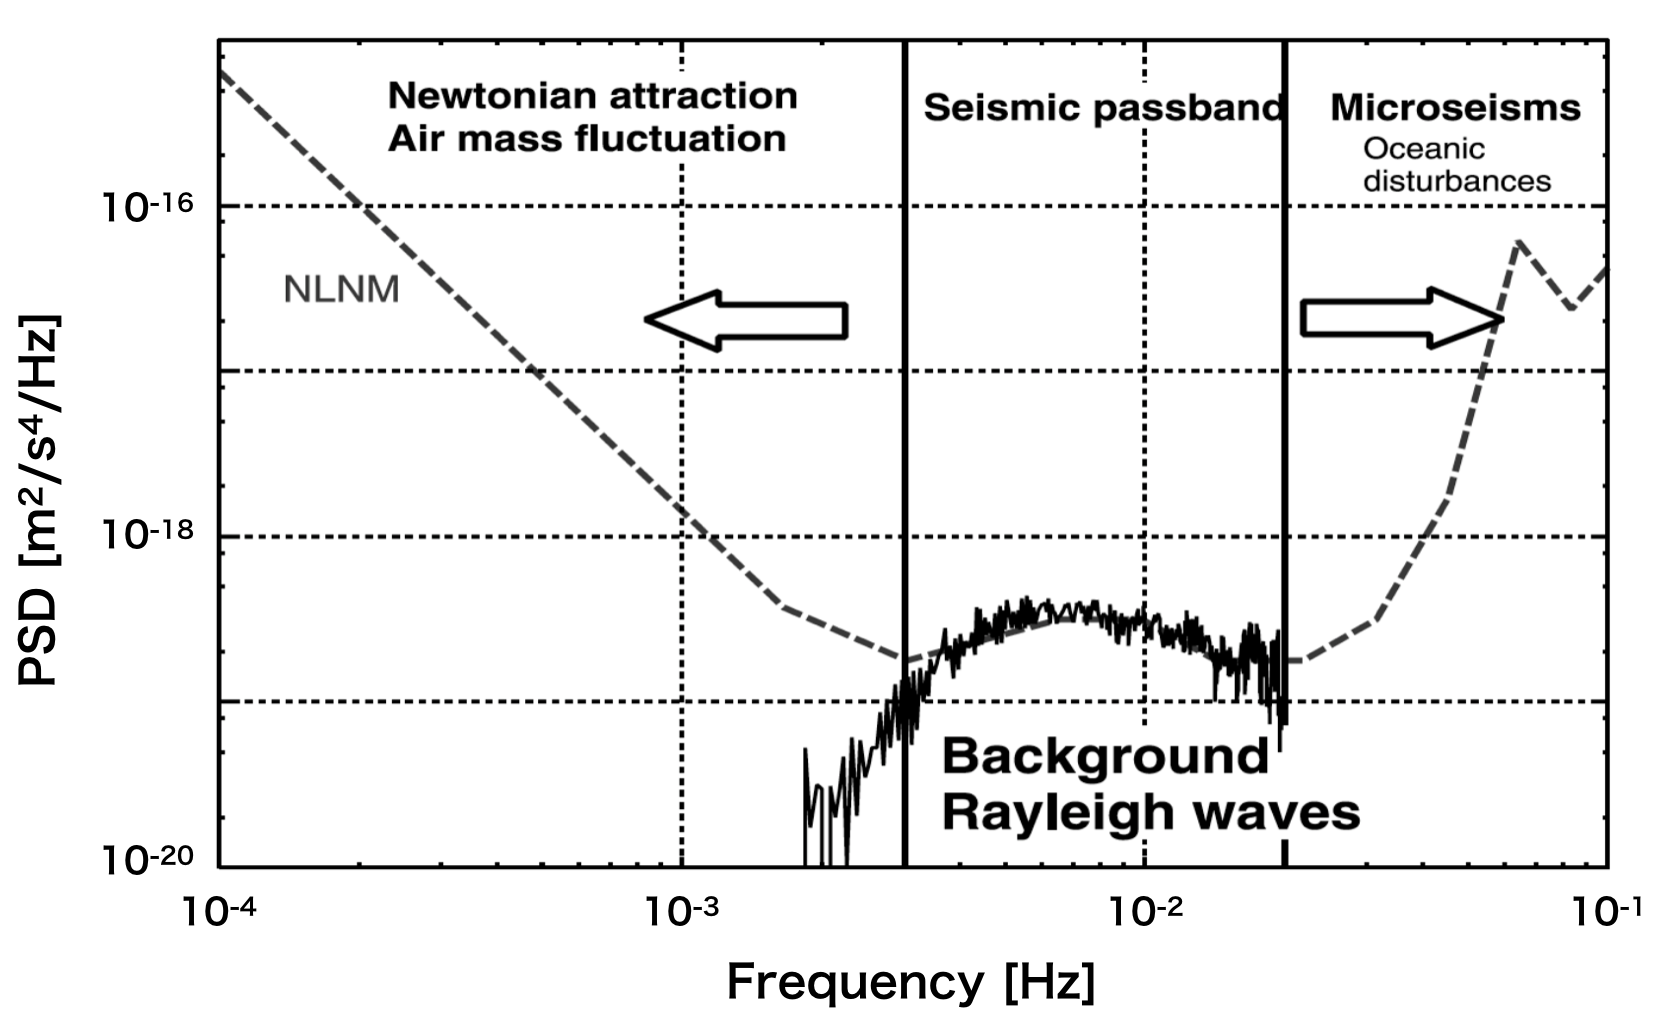
\includegraphics[width=12.5cm]{./img_chap3/img325.png}
    \caption{\cite{nishida2002origin}から転載。
    }\label{img:img325}
  \end{center} 
\end{figure}


\subsubsection{Microseisms}
Microseisms which power spectrum has peaks in $50$--$200\,\mathrm{mHz}$ are excitated by oceanic waves. These seismic waves can be categolized by the generating mechanism of these \cite{Bormann2012new}. First, the primary ocean microseisms are generated only in shallow waters in coastal regions. In this regions, the water wave enery can be converted directly into seismic energy either through vertical water pressure variations, or by the impacts of surf on the shores. There are correlation between this microseismic peak and the swell at the beaches was known starting from the data sets studied by \cite{haubrich1963comparative}. Second, the secondary ocean microseisms could be explained by the superposition of ocean waves of equal period traveling in opposite directions. Therefore, generating standing gravity waves of half the period \cite{longuet1950theory}.

The RMS amplitude spectral of both type of the microseisms are strongly depends on the low pressure on the ocean \cite{naticchioni2014microseismic}.

\subsubsection{Seismic Noise Below $20\,\mathrm{mHz}$}
Below the microseismic frequency band, the main seismic noise source is an atmospheric pressure change; Rayleigh waves excited by air fluctuation on the surface, and the deformation of the Earth's crust caused by the Newtonian attraction of air mass fluctuation \cite{sorrells1971earth,zurn1995noise}. Fig, \ref{img:img325} shows PSDs of the New Low Noise Model (NLNM) \cite{peterson1993observations} and the measured former noise \cite{nishida2002origin}, and the noise is consitent with the NLNM between $2\,\mathrm{Hz}$ and $30\,\mathrm{mHz}$. Moreover, the latter noise is increase PSD increases rapidly with decreasing frequency below 2 mHz. ここで特筆すべきは、2mHz以上のノイズはRayleigh waveで運ばれるため、地下に潜ればいくらか低減が期待されることである。実際に地表と地下のひずみ計による観測によってそれが示唆されている\cite{araya2007broadband}。

\subsubsection{Earth tides}
Below more lower frequency, the earth deformed by tidal forces due to the attraction of the Sun and the Moon in diurnal and semi-diurnal period. 

(なにかもう少し書く)

\subsubsection{Large Earthquake in the world}
大規模な地震ほど低周波の地面振動成分が卓越することが知られている\cite{aki2002quantitative,aki1967scaling}。地震によるサイトの地面振動は断層のズレ方と伝搬経路に依存するが、ここでは、同じ場所で同じ震源同じ断層のズレ方を前提とする。このとき以下のようなモデルが観測値をよく説明する。
\begin{eqnarray}
  s(\omega) = \displaystyle\frac{S_0}{1+({\omega}/{\omega_0})^2} 
\end{eqnarray}
ここで$M_{\mathrm{s}}$は表面波マグニチュードである\cite{gutenberg1945study}。そして$S_0$は$M_{\mathrm{s}}$に比例した定数で、$\omega_0$は$M_{\mathrm{s}}^{1/3}$に比例したコーナー周波数である。この変位スペクトルをさまざまな表面波マグニチュードでプロットしたものをFig(\ref{img:img328})に示す。

このように大規模地震は低周波の地面振動を励起しやすく、特に

\section{Study of Seismic Noise of KAGRA Mine} \label{sec:33}
\subsection{Overview}
KAGRAでは、我々は地面振動を地震計とひずみ計をつかったリアルタイムモニターシステムを構築している。このシステムの目的は、地面振動に最も敏感な腕共振器を懸架するTypeAサスペンションの地面振動をモニターすることである。そのため、我々は広帯域地震計であるTrillium120を3台、TypeAが懸架されているコーナーエリアと両エンドエリアの二階の地面に設置し、ひずみ計は現在Xアームに設置している。これらセンサーは自身のセンサーノイズの特性上、帯域を相補的に地面振動をモニターしている;0.1Hz以上は地震計で、1Hz以下はひずみ計でモニターしている。

本節ではこれらセンサーをつかって、KAGRAの地面振動ノイズの時間的空間的な特徴を調べた。

\subsection{Experimental Arrangement}\label{sec:331}
We used Trillium 120-QA which is known as three-component, very broadband, and low-noise seismometer. These three outputs are proportional to the ground velocity of two horizontal and one vertical, respectively. 

\begin{figure}[h]
  \begin{center}   
    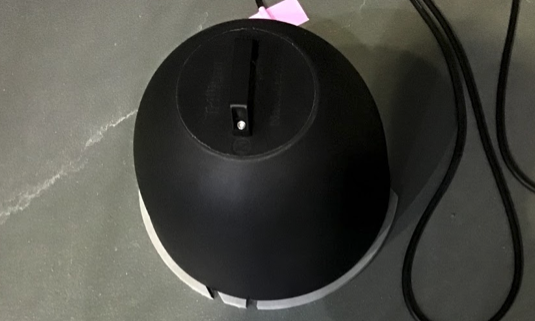
\includegraphics[width=9.0cm]{./img_chap3/img316.png}
    \caption{Trillium 120-QA installed on the second floor at X-end area, which is coverd by black thermal insulation cover}\label{img:img316}
  \end{center}
\end{figure}

The seismometer is housed in the black thermal insulation cover as shown in fig \ref{img:img316}. Thermal insulation protects two broad categories of thermal couplings that can cause unwanted noise \cite{trillium120manual}. First is the direct coupling to the sensitivity. This coupling typically increases the noise of the vertical channel as a periodic diurnal variation caused by the day-to-night temperature cycle, because the springs that suspended the inertial masses are temperature sensitive. The second is the coupling to tilt from the thermal fluctuation. Tilt converts the vertical acceleration of gravity into horizontal acceleration. This thermally induced tilt noise on the horizontal will be larger than the direct thermal coupling on the vertical channel. To be low sensitivity to both tilt and temperature, this model has a function to center the inertial mass after the initial installation.

The signals of the seismometer is recorded through the data aquisition system developed by LIGO \cite{bork2001overview}. The analog signal is converted to digital signal by the 16 bit analog-to-digital converters (ADC) with 16384 $\mathrm{Hz}$ sampling. This analog signal is amplified with 30 db so that the ADC noise does not mask this signal. 

\subsection{Data Processing}
振幅スペクトルの推定は50\%オーバーラップした32個のセグメントの平均で得た。それぞれのセグメントのFFTの計算は、まず dtrend をして線形成分を取り除き、Hanning窓にかけてから行った。32回の平均をおこなったスペクトルは自由度32のカイ二乗分布に従う。自由度$\nu$のときの$100(1-\alpha)$\%の信頼区間は、周波数$\mathrm{f}$でのスペクトルの推定量を$\hat{G}(f)$とすると、
\begin{eqnarray}
  \frac{\nu{\hat{G}(f)}}{\chi^2(\nu,1-\frac{\alpha}{2})} \leq G(f) \leq \frac{\nu{\hat{G}(f)}}{\chi^2(\nu,\frac{\alpha}{2})}
\end{eqnarray}
で与えられる。したがって、95\%の信頼区間は
\begin{eqnarray}
  \nu/\chi^2(\nu,1-\frac{\alpha}{2}) \leq G(f)/\hat{G}(f) \leq \nu/\chi^2(\nu,\frac{\alpha}{2})
\end{eqnarray}
となり、自由度32の場合、推定量の0.65 から1.75 の範囲になる。

\subsection{Study of Long-term Seismic Noise}
Long-term seismic noise is measured by a seismometer installed on the second floor of the X-end area. This area is placed 200 $\mathrm{m}$ underground from the surface of the mountain. In comparison to corner area, human activity in the end area is less because the corner area has parking lots. In comparison to the Y-end area, there is no entrance connected to other mines. Therefore, the X-end area is relatively quiet in the KAGRA mine, regarding the seismic noise induced by human activity. 

地震や回路からの突発的なノイズを含まない一年間のデータをつかって、ノイズスペクトルを計算した。並進成分と垂直成分両方の加速度のASDをFigure \ref{img:img313}に示す。40mHz以上では並進成分も垂直成分も同じ振幅スペクトル密度をもつ。40mHz以下で並進成分が垂直成分よりも大きいが、これは付録で後述しているとおり、無相関なノイズである。おそらく温度ゆらぎから生じる傾斜カップリングだと考えられる。また、Petersonのスペクトルと測定で得た10パーセンタイルを比較すると、0.1から2Hzをのぞいて、NLNMと同じである。0.1Hz以下では垂直成分は地面振動のノイズレベルと同等であり。2Hz以上は、並進も垂直成分も、地下環境のおかげで静かである。対照的に0.1から2Hzの帯域では、並進成分も垂直成分もNLNMより数倍大きい。これはKAGRAが富山湾から40kmの距離にあり、比較的脈動の影響を受けやすいためと考えられる。
\begin{figure}[p]
  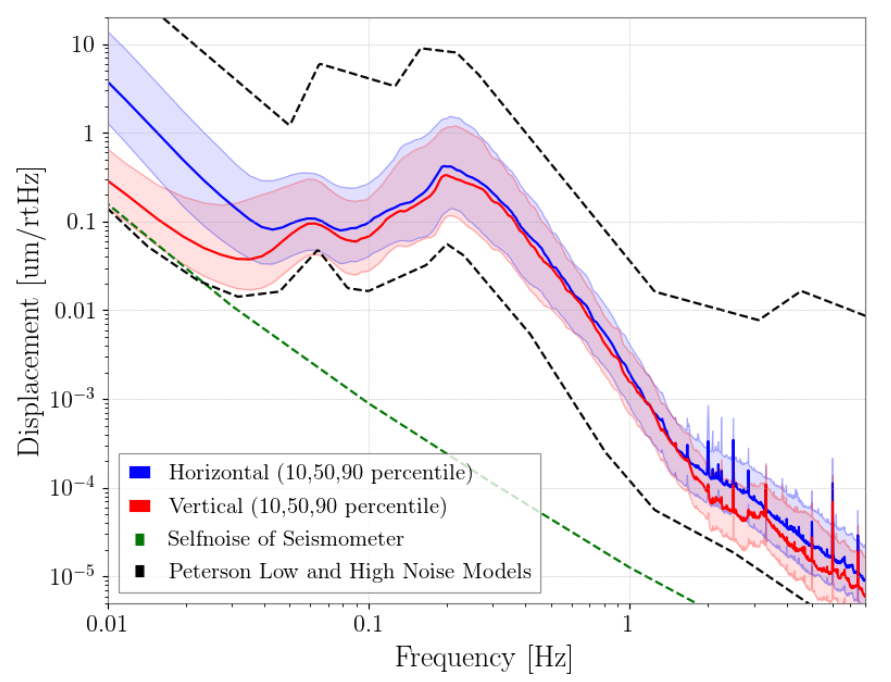
\includegraphics[width=13.0cm]{./img_chap3/img313.png}
  \caption{赤の実線は垂直成分の50パーセンタイルで、下と上に10と90パーセンタイルを示す。青の実線はX軸とY軸の二乗和から求めた並進成分であり、同様に10,50,90パーセンタイルを示す。緑点線はTrillium120 のデータシートから引用したSelfnoiseである。黒の点線はPetersonのNLNMとNHNMである。}\label{img:img313}
\end{figure}

\subsection{Study of the Differential Motion Reduction} \label{sec:332}

\subsubsection{CDMR in X-arm }
\cref{sec:313}でのべたCDMRの効果を, Xアームの両端においた地震計2台をつかって評価した。


\begin{figure}[p]
    \begin{center}   
      
\includegraphics[width=13.0cm]{./img_chap3/img319.png}
      \caption{Comparison with the measured CDMR and the uniform plane waves model. (Top) ASDs of the velocity of the differencial (solid line) and common motion (dashed line) of the baseline used calculating the below CDMR. Red and blue indicate X-arm and Y-arm, respectively. As a comparison to these ASDs, black dashed line shows the seilfnoise of the Trillium 120Q broadband seismometer multiplied $\sqrt{2}$. Below 0.05 Hz, the ASDs are limited by the noise mentioned in section \cref{sec:331}. (Bottom) The CDMR of the baseline calculated with the differential and common motion of the baseline according to  the definition in Eq.(\ref{eq:eq23}). Glay line indicates the CDMR assuming the uniform plane waves model in case the phase velocity is in region from 5 -- 3 km/sec. Green dashed line is the CDMR assuming the no correlation between the each end points of the baseline. The measured CDMR is consistent with the uniform model in 0.05 -- 0.5 Hz. Below this band, the CDMR is close to the no correlation model due to the noise of the seismometers. Above this band, }\label{img:img319}
    \end{center}
\end{figure}


\subsubsection{基線長の違いによるCDMRの変化}
aaa

\begin{figure}[p]
  \begin{center}
    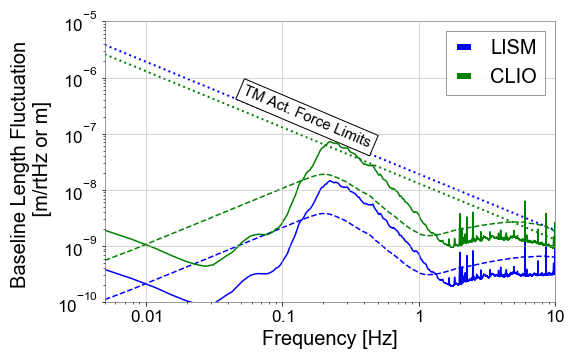
\includegraphics[width=12.5cm]{./img_chap3/img330.png}
    \subcaption{}\label{img:img330}
    \label{img:img327}    
    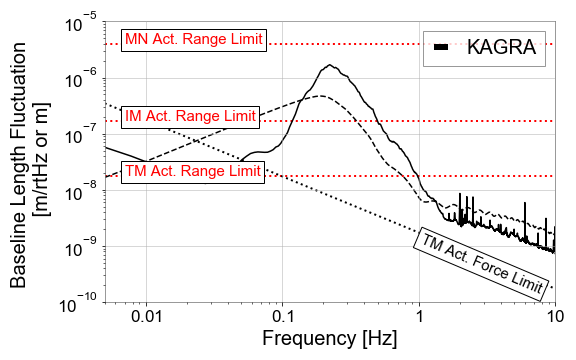
\includegraphics[width=12.5cm]{./img_chap3/img327.png}
    \subcaption{Comparison between the baseline length fluctuations and the displacement requirement of the underground GW detectors. Solid line is the baseline length fluctuation of the detectors, which is the ASD of the seismic noise (described in section \cref{sec:33}) multiplied by the function in Eq. \ref{eq:eq3} assumming the uniform plane wave model with the phase velocity of $3\,\mathrm{km/sec}$. Morever, dashed line is the accumulated RMS of the fluctuations. As a comparison, the displacement requirement of the detector, which is the linewidth of the arm cavity, is ploted. }\label{img:img327}
    \label{img:img327}
  \end{center}
    \caption{aa}  
  \begin{center}
    \captionof{table}{Comparison of the underground GW detectors}  
    \begin{tabular}{lll} 
      \hline      
      Detector & Baseline length [m] & Linewidth [um] \\ \hline \hline
      LISM  & 20   & 0.1 \\
      CLIO  & 100  & 0.1 \\
      KAGRA & 3000 & 0.1 \\      
    \end{tabular}
    \label{tb:31}
  \end{center} 
\end{figure} 



\section{Summary of the Chapter}
 % Underground Seismic Noise
%% \chapter{Geophysics Interferometer (GIF)}



\section{Introduction}
地物干渉計の目的は、地球物理学の現象を精密に測定することと、KAGRAの基線長をモニターすることである。
\subsection{Laser Strainmeter for Geophysics}



\subsection{Motivation in GW detectors}


\section{Working Principle}

\subsection{Asynmetric Michelson Interferometer}

\begin{eqnarray}
  \phi = 2\pi\frac{2(l_x-l_y)}{\lambda}\sim4\pi\frac{l_x}{\lambda}
\end{eqnarray}

\begin{eqnarray}
  |d\phi| = 4\pi\frac{l_x}{\lambda}\left( \left|\frac{d\lambda}{\lambda}\right| + \left|\frac{dl_x}{l_x}\right| \right)
\end{eqnarray}


\subsection{Response to the seismic strain}
\begin{figure}[h]
  \begin{center}
    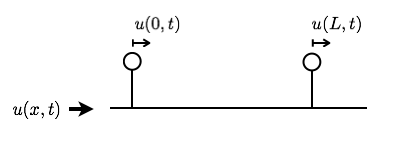
\includegraphics[width=10.0cm]{./img_chap4/img410.png}
    \caption{The displacements of the two points which are sparated L in X axis. }
  \end{center}
\end{figure}

The response of the strainmeter to seismic waves have characteristics of the low pass filter. To calculate this response, it is assumed that the plane seismic waves which displacement $u(x,t)$ is represented as $u(x,t)=u_0e^{i(\omega{t}-kx)}$ with angular frequency of $\omega$ and wave number of $k$, propagate along with the direction of the base-line of the strainmeter. The length fluctuation between two mirrors sparated with $L$ can be expressed as 
\begin{eqnarray}
  \Delta{L(t)} &\equiv& u(0,t) - u(L,t) \\
  &=& u(0,t) - u(0,t-\tau), \label{eq:chap4_10}
\end{eqnarray}
where $\tau=L/v$ is the time delay. 
The transfer function from the displacement to the length fluctuation is
\begin{eqnarray}
  H_{\mathrm{disp}}(s) \equiv \frac{\Delta{L(s)}}{u(s)} = 1 - \exp(-\tau{s})
\end{eqnarray}

Because the strain amplitude $\epsilon(x,t)$ is defined as $\epsilon(x,t)\equiv\frac{du}{dx}$, the strain
\begin{eqnarray}
  \epsilon(x,t) \equiv \frac{du}{dx} &=& \frac{du}{dt} \frac{dt}{dx}\\
  &=& {u(x,t)}^{\prime}\frac{1}{v}
\end{eqnarray}


Therefore, the response of the strainmter to the seismic strain is given

\begin{eqnarray}
  H_{\mathrm{strain}}(s) \equiv \frac{\Delta{L(s)}}{\epsilon(s)} = \frac{\Delta{L(s)}}{\frac{s}{v}u(s)} = \left(1 - \mathrm{exp}(-\tau{s})\right) \frac{v}{s}
\end{eqnarray}



\begin{figure}[h]
  \begin{center}
    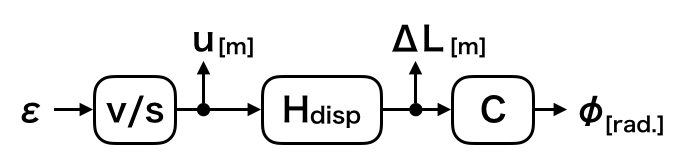
\includegraphics[width=10.0cm]{./img_chap4/img411.png}
    \caption{}
  \end{center}
\end{figure}


\begin{figure}[h]
  \begin{center}
    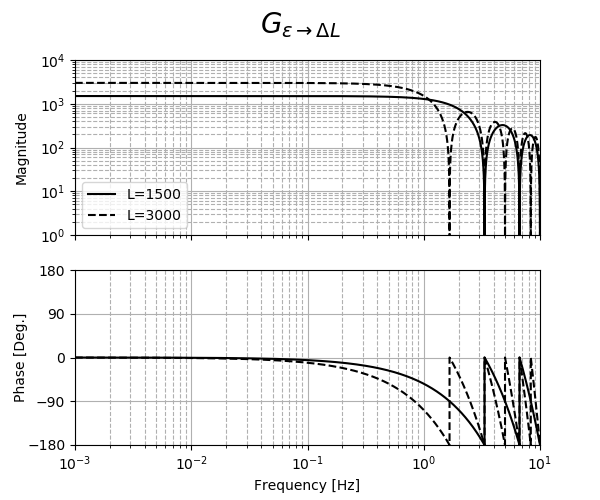
\includegraphics[width=12.0cm]{./img_chap4/img412.png}
    \caption{Transferfunction from strain of the baseline ($\epsilon$) to the length change of that ($\Delta{L}$). }
  \end{center}
\end{figure}


\subsection{Signal Detection Scheme}
\subsubsection{Quadrature Phase Detection}


\subsection{Noise}


どういうノイズが原理的に存在するか述べる。空気ゆらぎ、周波数雑音を述べる。


\section{Optics Design} %光学系
...\\
\subsection{Overview}
Optical layout is shown in Fig. \ref{img:img}. Optics of GIF is categorized by three category; mode-matching optics, core optics and frequency stabilized laser.

\begin{figure}[h]
  \begin{center}   
    
\includegraphics[width=9.0cm]{./img.png}
    \caption{}\label{img:img}
  \end{center}
\end{figure}


\subsection{Design Concept}
設計で考慮しなければならない点は
*干渉位置で2つのモードが合っていること
*できるだけ光学系は小さくすること
である。

腕の長さから生じるモードのズレを小さくするために、エンドリフレクタでビームウエストを持つようにする。

\subsection{Input Output Optics}

\subsection{Core Optics}

\subsection{Frequency Stabilized Laser}

\section{Data Aquisition System}
\subsection{Realtime Processing}
\subsection{...}



\section{Summary of the Chapter} %章のまとめ
本章で述べたパラメータを表にまとめる。
 % Geophysics InterFerometer
%% \chapter{Baseline Compensation System}
Baseline compensation system is a one of the active vibration isolation system for GW detector's arm cavity. 

In the section \cref{sec:51}, the passive viblation isolation is described. After that, two type of active vibration isolation system are described in the section \cref{sec:52} and \cref{sec:53}. In the section \cref{sec:54}, the baseline compensation system is described.

\section{Basics in Seismic Isolation}\label{sec:51}
Essentialy, the vibration isolation system has a pendulum to attenuate the seismicnoise passively. For further the isolation performance, the pendulum have developed as a longer and multi-stage pendulum.

\subsection{Single Pendulum}
For simple example, as shown in left figure in Figure(\ref{img:img501}), consider a one-dimentional harmonic oscillator consisting of a spring with a spring constant $k$ and mass $M$. The displacement of the suspension point and the mass are $x_0$ and $x$, respectively. Because the equation of the motion is written as
\begin{eqnarray} \label{eq:eq501}
  M\ddot{x} = -k(x-x_0),
\end{eqnarray}
the frequency transfer function from the displacement of the suspension point to the mass displacement $H(f)$ is given by the Fourier transform from the equation and represented as
\begin{eqnarray} \label{eq:eq502}
  H(f) \equiv \frac{1}{1-(f/f_0)^2},
\end{eqnarray}
where $f_0 = (k/M)^{1/2}$ is the resonant angular frequency of the oscillator.

According to Eq.(\ref{eq:eq502}), the amplitude of $H(f)$ is unity below the resonant frequency, the amplitude is approximately propotional to $(f/f_0)^{-2}$ above resonance frequency. The bode plot of $H(f)$ with various resonance frequencies are plotted in right figure in Figure \ref{img:img501} . One finds that it is better to make a low-resonance frequency oscillator in order to attenuate the seismic noise broadly. 

\begin{figure}[h]
  \begin{center}   
    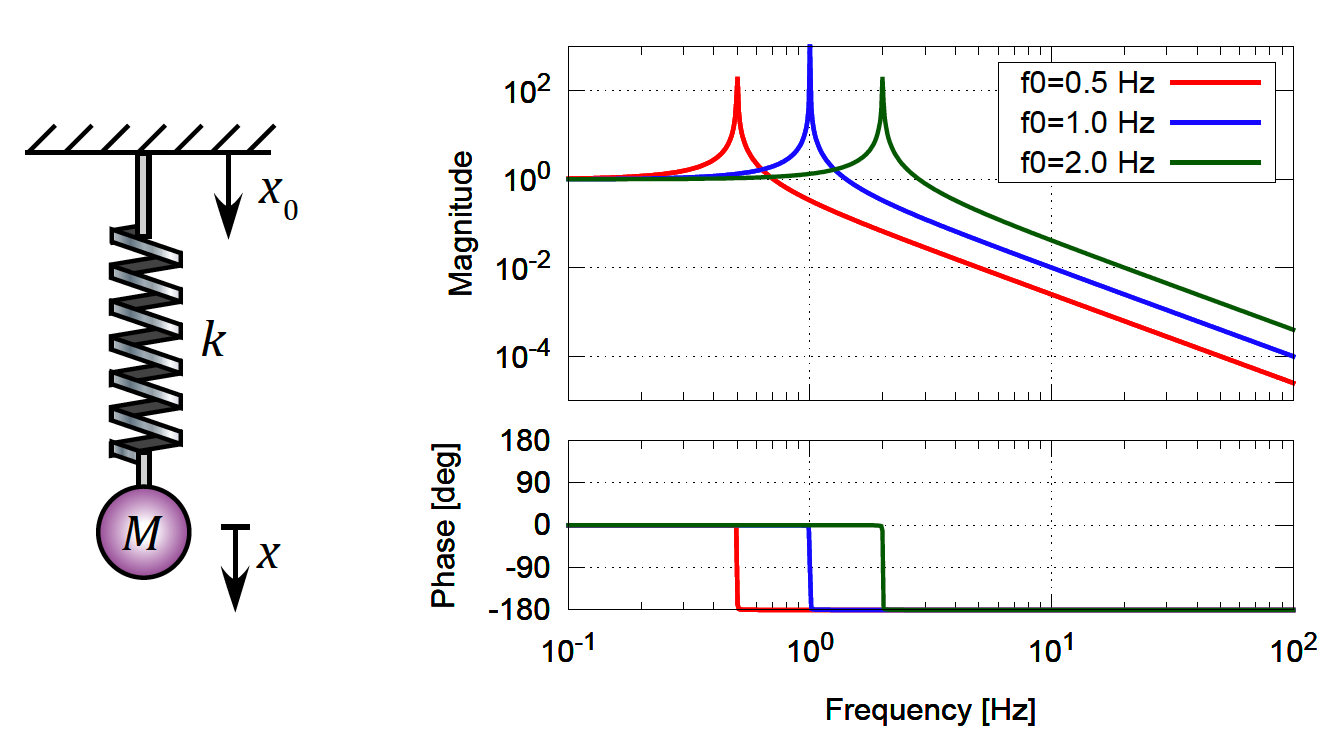
\includegraphics[width=11cm,height=6cm]{./img_chap5/img501.png}
    \caption{Single pendulum as a mechanical filter and its transfer function with various resonant frequencies. This figure is cited from Figure(2.3) in \cite{sekiguchi2016astudy}.} \label{img:img501}
  \end{center}
\end{figure}

\subsection{Multi-stage Pendulum}
In order to increase the order of the seismic isolation, multi-stage pendulum is effective. In case of an N-stage pendulum, the transfer function from the ground to the suspended mass is propotional to $f^{-2N}$ above the resonance frequrncy of the pendulum as shown in Figure \ref{img:img502}. 
\begin{figure}[h]
  \begin{center}   
    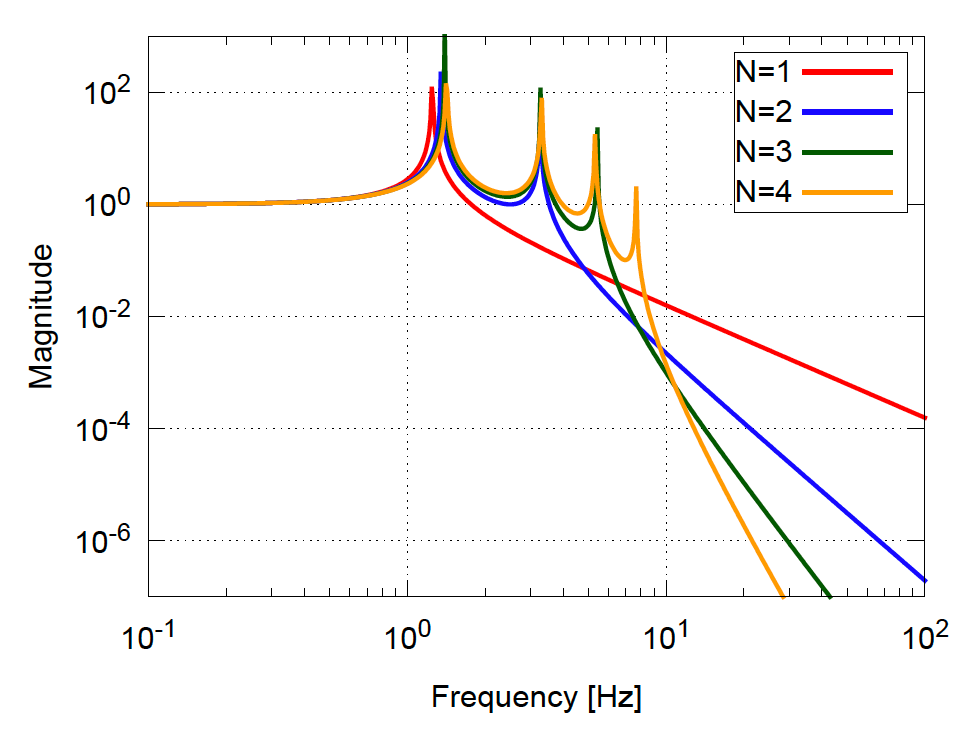
\includegraphics[width=10cm,height=7cm]{./img_chap5/img502.png}
    \caption{The amplitude of the transfer function of the N-stage pendulum. This figure is cited from Figure 2.4 in \cite{sekiguchi2016astudy}.} \label{img:img502}
  \end{center}
\end{figure}


\section{Active Inertial Seismic Isolation}\label{sec:512}
\begin{figure}[h]
  \begin{center}
    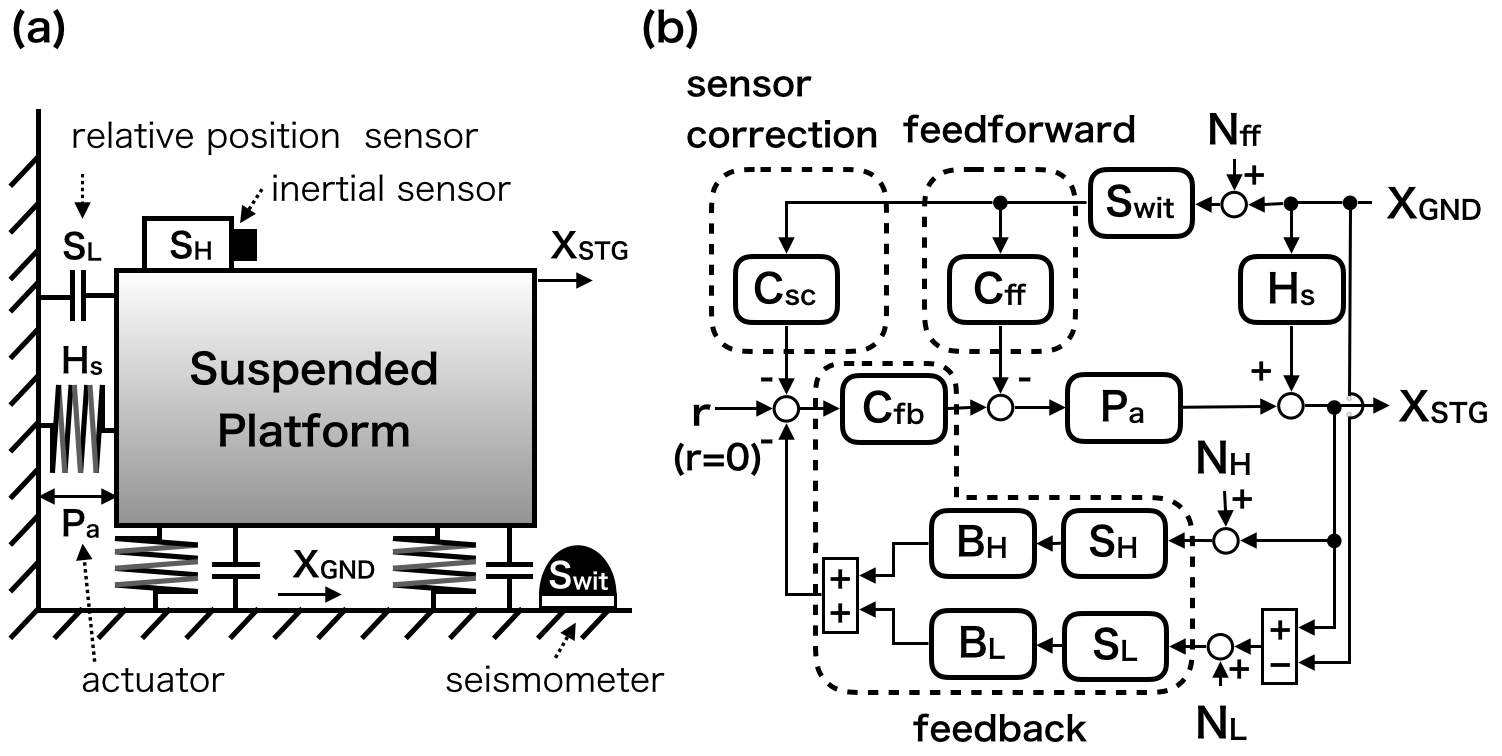
\includegraphics[width=13.5cm]{./img_chap5/img503.png}
    \caption{{\bf(a)} Schematic drawing of an active seismic isolation system for platform. {\bf(b)} Block diagram of the active control scheme.} \label{img:img503}
  \end{center}
\end{figure}
The passive vibration isolation cannot reduce the seismic noise below its pendulum's eigenfrequency. To attenuate the lower-frequency seismic noise, the active vibration isolation system using a seismometer \cite{matichard2015seismic}.

The active isolation system is shown in Figure \ref{img:img503}(a). A platform is suspended from the ground with transmisivity $H_{\mathrm{s}}$. This platfrom is fed back both signal of a inertial sensor with calibration factor $S_{\mathrm{H}}$ and signal of a relative position sensor with calibration factor $S_{\mathrm{L}}$, to the platform using actuator with actuator efficiency $P_{\mathrm{a}}$. This feedback control actively decouple the platform from the seismic disturbance from $0.1\,\mathrm{Hz}$ to a few Hz. Moreover, the platform is controled with feedforward using a seismometer with calibration factor $S_{\mathrm{wit}}$ installed on the local ground. 

As shown in Figure \ref{img:img503}(b), the active vibration system is integrated with a feedback control, sensor correction contorl, and feedforward control. These control schemes are described below.

\subsection{Sensor Blending Technique}
\begin{figure}[h]
  \begin{center}   
    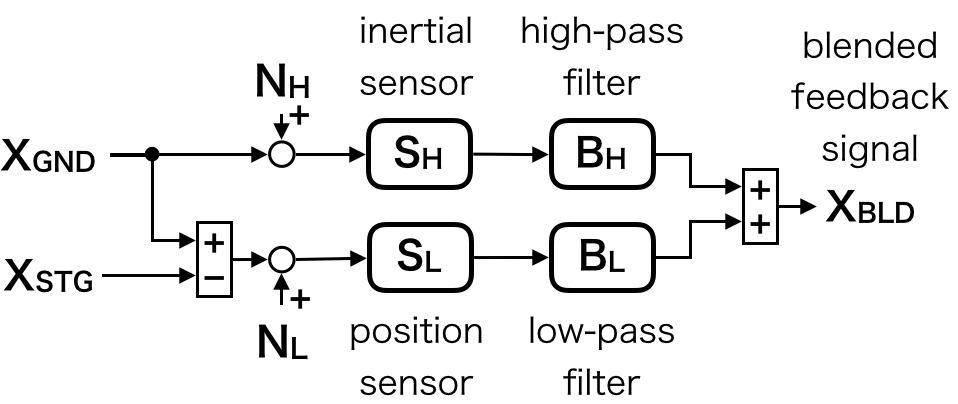
\includegraphics[width=10cm]{./img_chap5/img507.png}
    \caption{Sensor Blending.} \label{img:img507}
  \end{center}
\end{figure}

The purpose of the active inertial seismic isolation is to reduce the stage motion against the inertial frame. Thus, we use the feedback control using a inertial sensor. However, because the noise level of the inertial sensor is worse in low-frequency regison, the feedback system cannot use the inertial sensor in this region. Nevertheless, to control the DC position of the stage. In this situation, the sensor blending technique is commonly used in the active viblation system.

As shown in Figure \ref{img:img507}, the feedback signal is belended by singals of the inertial and position sensors. The inertial sensor output is filterd with high-pass filter $B_{\mathrm{H}}$ because noise of the sensor is worse in low-frequency region. On the other hand, the position sensor is filterd with a filter $B_{\mathrm{L}}$ so that
\begin{eqnarray}
  B_{\mathrm{H}}S_{\mathrm{H}} + B_{\mathrm{L}}S_{\mathrm{L}} = 1,   \label{eq:eq506}
\end{eqnarray}


In the case of using the blended feedback signal, the displacement of the platform stage. The displacement of the stage is given by
\begin{eqnarray}
  X_{\mathrm{STG}} = \frac{G}{1+G}LX_{\mathrm{GND}} + \frac{1}{1+G}H_{\mathrm{s}}X_{\mathrm{GND}} + \frac{G}{1+G}\left(HN_{H}+LN_{L}\right),   \label{eq:eq510}
\end{eqnarray}
where $X_{\mathrm{STG}},\,X_{\mathrm{GND}},\,N_{\mathrm{H}},$ and $N_{\mathrm{H}}$ are the displacement of the stage and the ground motions, and the noise of the inertial sensor and the position sensor, respectively. Moreover $G=C_{\mathrm{fb}}P_{\mathrm{a}}$ is the loop gain, and the multiples of the comprimentary filters and each sensor responses are defined as $L=B_{\mathrm{H}}S_{\mathrm{H}}$ and $H=B_{\mathrm{L}}S_{\mathrm{L}}$, respectively. Here, if the feedback is work enough, thus the loog gain is large enough, the displacement of the stage is given as
\begin{eqnarray}
  \lim_{G\to\infty} X_{\mathrm{STG}} = LX_{\mathrm{GND}} + \left(HN_{H}+LN_{L}\right) \label{eq:eq510_a}
\end{eqnarray}

According to Eq.(\ref{eq:eq510_a}), to isolate the stage against the inertial frame, the active isolation system should design $L$ as small as possible, whereas the $H$ as the complementary filter of that must be large, which means that the inertial sensor noise introduce to the stage. Actually, the cutoff frequency of these filters are choosed at $100\,\mathrm{mHz}$ due to the inertial sensor noise, and the system cannot isolate the seismic noise below this frequency. In other words, although the active vibration syste using the inertial sensor can design the response from the ground to the stage by filter $L$, the system performance is limited by the inertial noise in low-frequency region.

\subsection{Sensor Correction Technique}
\begin{figure}[h]
  \begin{center}   
    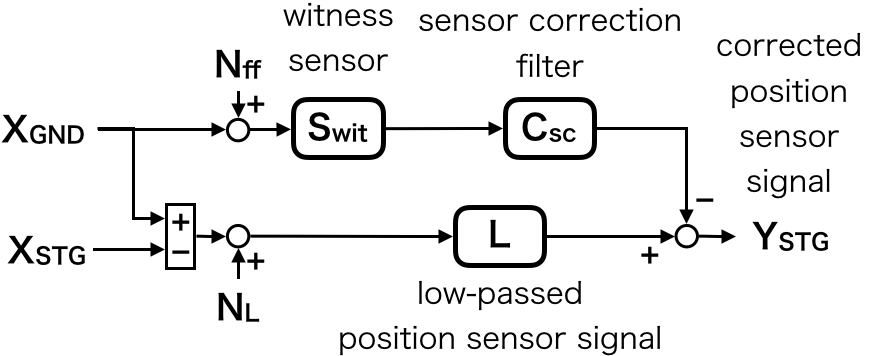
\includegraphics[width=10cm]{./img_chap5/img505.png}
    \caption{Sensor correction scheme.} \label{img:img505}
  \end{center}
\end{figure}
Sensor correction technique is a method to correct the posision sensor using the additional inertial sensor on the ground \cite{hua2005low}. As mentioned above, because of the insufficient noise of the inertial sensor on the stage, the blended feedback signal use had to use the position sensor in the low-frequency. This means that the stage motion is reduced to the local ground frame not inertial frame in this frequency region. Thus, the sensor correction remove the groung motion from the position sensor by using anothor seismometer on the ground that have better sensitivity than the inertial sensor on the stage. The corrected feedback signal can compensate the performance of the inertial sensor on the stage.

Consider the displacement of the vibration isolated stage utilizing sensor correction technique. As shown in Figure\ref{img:img503}, the correction signal from the seismometer signal is injected at the set-point through the control filter $C_{\mathrm{sc}}$ to remove the ground motion from the feedback signal using the position sensor. The displacement of the stage is given by 
\begin{eqnarray}\nonumber
  X_{\mathrm{STG}} &=&\frac{G}{1+G}L\left(1-C_{\mathrm{sc}}\frac{S_{\mathrm{wit}}}{L}\right) X_{\mathrm{GND}} + \frac{1}{1+G}H_{\mathrm{s}}X_{\mathrm{GND}}\\ 
  &+& \frac{G}{1+G}\left(HN_{H}+LN_{L}\right) + \frac{G}{1+G}C_{\mathrm{sc}}S_{\mathrm{wit}}N_{\mathrm{ff}} \label{eq:eq511}
\end{eqnarray}
Here, in the case that the loop gain is large enough, the stage motion is given by 
\begin{eqnarray}
  \lim_{G\to\infty} X_{\mathrm{STG}} = L\Delta_{\mathrm{sc}} X_{\mathrm{GND}} + \left(HN_{H}+LN_{L}\right) + {L}N_{\mathrm{ff}} \label{eq:eq513},
\end{eqnarray}
where 
\begin{eqnarray}
  \Delta_{\mathrm{sc}} \equiv \left(1-C_{\mathrm{sc}}\frac{S_{\mathrm{wit}}}{L}\right) \label{eq:eq512}
\end{eqnarray}
is the gain matching coeffient. By comparison with Eq.(\ref{eq:eq513}) and Eq.(\ref{eq:eq510_a}), the displacement of the stage can be reduced by the gain matching.

Although this gain maching factor can be zero when $C_{\mathrm{sc}}=B_{\mathrm{L}}(S_{\mathrm{wit}}/S_{\mathrm{L}})$, actually, the factor is limited by the caliblation errors of the witness sensor and the inertial sensor on the stage. At least, the error can not be less than 5\%, so it is difficult to achieve the vibration isolation ratio of 20 \cite{hua2005low}.

\subsection{Feedforward Technique}
\begin{figure}[h]
  \begin{center}   
    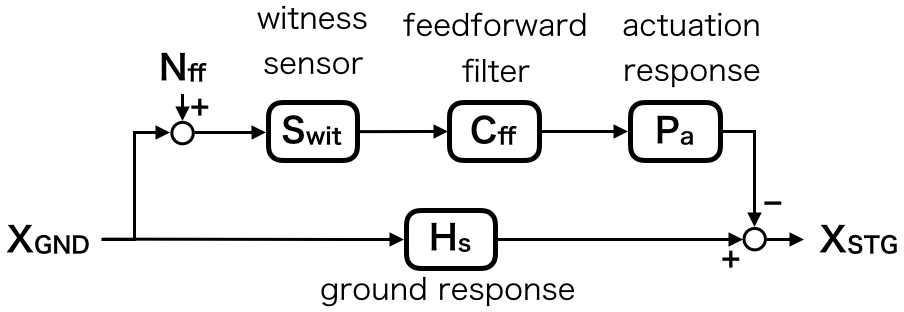
\includegraphics[width=10cm]{./img_chap5/img506.png}
    \caption{Feedforward scheme.} \label{img:img506}
  \end{center}
\end{figure}
Feedforward technique is similar to sensor correction, but this technique remove the motion caused by the ground motion directly. Figure\ref{img:img506} shows the block diagram of the feedfoward control. While the stage motion $X_{\mathrm{STG}}$ is disturbed by the ground motion $X_{\mathrm{GND}}$ through the mechanical response of the platform $H_{\mathrm{s}}$, the feedforward compensates the stage motion by subtracting the disturbance with the witness sensor (in this case, seismometer) signal. This feedforward control does not depend the feedback control unlike the sensor correction. In other words, the feedforward control works in the frequency region where the feedback loop gain is small, whereas the sensor correction works in the high loop gain region. Therefore, both feedforward and sensor correction technique is used to improve the vibration isolation system in all frequency region.


Finally, consider the control integrated with three techniques; sensor blending, sensor correction, and feedforward. In the case that the additional feedforward signal is injected at the error-point, as shown in Figure \ref{img:img503}, the displacement of the stage motion is given by
\begin{eqnarray}\nonumber
  X_{\mathrm{STG}} &=&\frac{G}{1+G}L\Delta_{\mathrm{sc}} X_{\mathrm{GND}} + \frac{1}{1+G} \Delta_{\mathrm{ff}} X_{\mathrm{GND}}\\ \nonumber
  &+& \frac{G}{1+G}\left(HN_{H}+LN_{L}\right) + \frac{G}{1+G}C_{\mathrm{sc}}S_{\mathrm{wit}}N_{\mathrm{ff}} \\ 
  &+& \frac{1}{1+G}P_{\mathrm{a}} C_{\mathrm{ff}}S_{\mathrm{wit}}N_{\mathrm{ff}} \label{eq:eq514}.
\end{eqnarray}
Here, 
\begin{eqnarray}
  \Delta_{\mathrm{ff}} \equiv \left(H_{\mathrm{s}}-P_{\mathrm{a}}C_{\mathrm{ff}}S_{\mathrm{wit}}\right) \label{eq:eq515}
\end{eqnarray}
is defined as the gain matching coefficient of the feedforward. One can find that, in  Eq.(\ref{eq:eq514}),  the first and second terms indicating the contribution from the ground motion can be reduced by the gain matching factors: $\Delta_{\mathrm{sc}}$ and $\Delta_{\mathrm{ff}}$. This reduction works independant from the feedback loop gain.

\subsection{Problem in Tilt-Horizontal Coupling}
The inertial sensors have problem in horizontal measurement in low-frequency due to a coupling from the tilting. This is called the tilt-horizontal coupling. Because of this coupling the feedback control using the inertial sensor cannot suppress the horizontal seismic motion aggressivly.

\subsubsection{Tilt-horizontal coupling}
\begin{figure}[h]
  \begin{center}   
    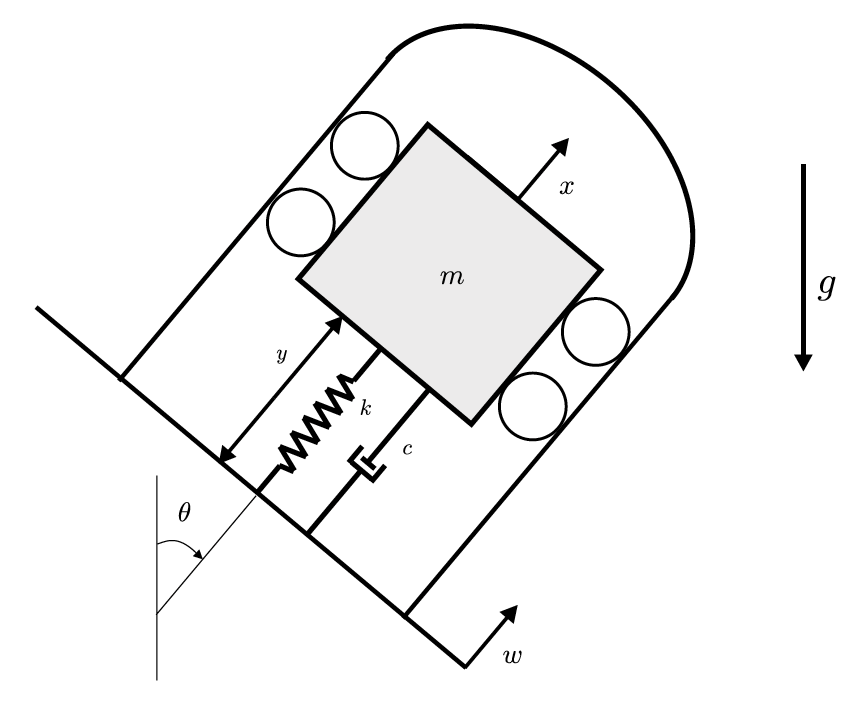
\includegraphics[width=8cm]{./img_chap5/img509.png}
    \caption{Tilted inertial sensor. Cited from Figure12 in \cite{collette2012inertial}} \label{img:img509}
  \end{center}
\end{figure}
 The inertial sensors cannot distinguish the horizontal or tilt motions of the ground because the inertial sensor measure the apparent force from the sensor frame. This coupling is known as the tilt-holizontal coupling and the response from each ground motion is given by \cite{collette2012inertial}
\begin{eqnarray}
  Y(s)=\frac{-m s^{2}}{m s^{2}+c s+k} \left[ W(s) + \frac{g \sin \left(\theta_{0}\right)}{s^2} \Theta(s) \right] \label{eq:eq515},
\end{eqnarray}
where $W(s),\,Y(s)$, and $\Theta(s)$ are, Laplace transformed, the displacement of the mechanical oscillator in the sensor, the relative displacement of the oscillator and the house enclosuring it, and the tilting angle of the house, respectively. Moreover, $m,\,c,\,k,\,g,$, and $\theta_0$ are the mass of the osclillator's proof mass, viscous damping coefficient, spring constant, and gravitational acceleration. According to Eq.(\ref{eq:eq515}), when 
\begin{eqnarray}
  f < \sqrt{\frac{g\sin(\theta_0)}{(2\pi)^2}}\ [\mathrm{Hz}]
  \label{eq:eq515}
\end{eqnarray}
the tilt motion tends to couple to the horizontal motion. For example, in the case of the maximum tilt coupling: $\theta_0=\pi/2$, the tilt motion contaminates the horizontal motion when $f<0.5\ [\mathrm{Hz}]$.

\subsubsection{Control strategy to avoid the problem}
As described above, the inertial sensor cannot be used for measuring the horizontal motion because of the inertial sensor behaving the tilt sensor. For the reason, the active inertial seismic isolation system in LIGO use the tilt sensor to remove the tilt components in the inertial sensor for avoiding the tilt-horizontal problem \cite{biscans2018optimization}.


\section{Active Baseline Seismic Isolation}
For laser interferometric gravitational-wave detector, the baseline length should be isolate from the seismic noise, whilie it is not necessary to isolate the individual stages to the inertial frame. For this reason, the active baseline seismic isolation system using additional interferometer named suspension point interferometer (SPI) have been developed.

\subsection{Suspension Point Interferometer (SPI)}
The basic idea of the active baseline vibration isolation is proposed by Drever in 30 years ago. In this idea, the baseline length is kept by feedback or feedforward with the baseline length singal measured by the suspension point interferometer (SPI), which is installed near the suspension point of the pendulum to measure the length \cite{drever1987outline}. The advantage of this active vibration isolation system is the sensitivity of the SPI, which is better than that of the inertial sensor in low-frequency. Owing to this sensitivity, the system could attenuate the seismic noise to DC changes. Therefore, various type of the vibration isolation system have been deveolped so far.

\subsubsection{Fabry-Perot Optical Cavity Type }
\begin{figure}[h]
  \begin{center}   
    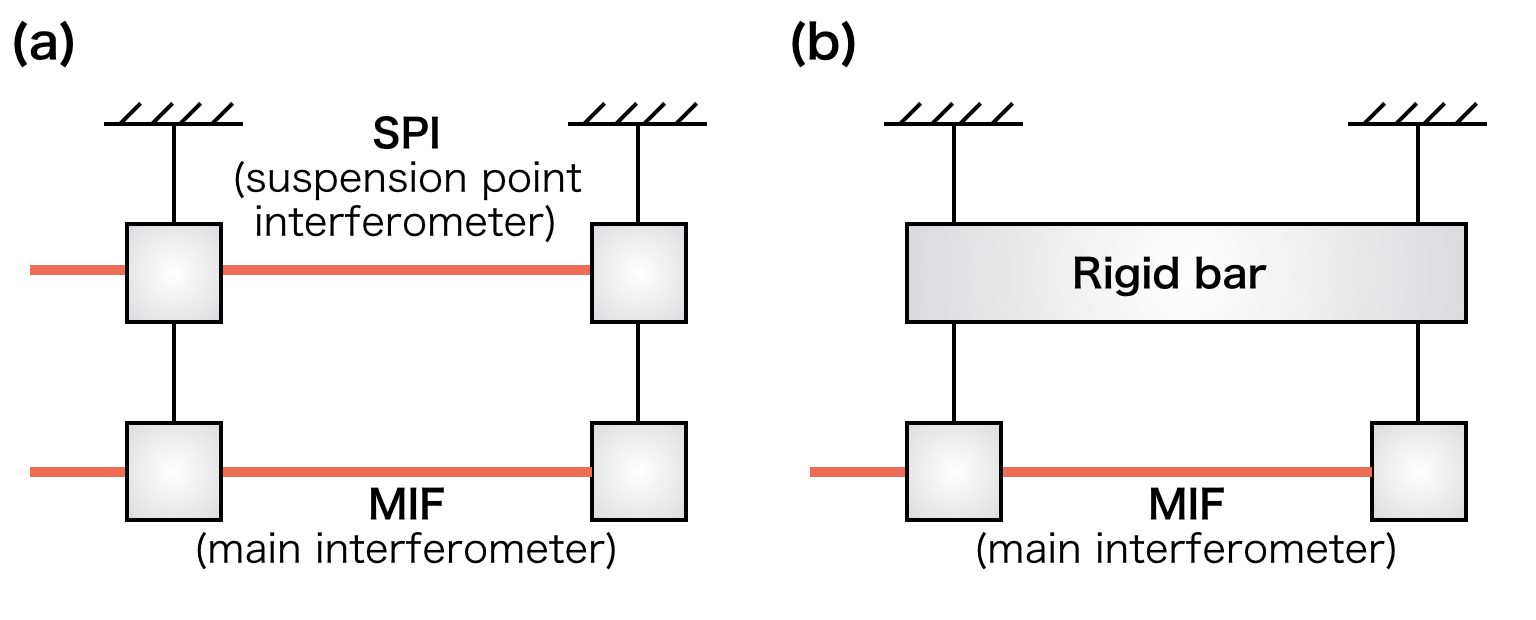
\includegraphics[width=13cm]{./img_chap5/img508.png}
    \caption{Schematic arrangement for one arm of SPI.} \label{img:img508}
  \end{center}
\end{figure}
Initial type of the SPI is, as shown in Figure \ref{img:img508}, the Fabry-perot optical cavity on the main interferometer's arm cavity \cite{drever2002extension}. The advantage of this idea is that this sytem can suppress the baseline length fluctuation using the feedback control because the SPI is installed near the main interferometer. Thus, if we increase the feedback gain, the length of the SPI behaves as the rigid bar as shown in Figure \ref{img:img508}(b). This means that the main cavity is suspended by the single pendulum from the ground, which does not change the baseline length entirely. Soon, 2 m proto type of SPI was developed and demonstrated about 40 db of vibration attenuation below 1 Hz \cite{aso2004stabilization}.

In general, the disadvantage of SPI is the noise coupling from the common motion due to the worse common mode rejection (CMR) above the eigenfrequency of the pendulums, because the active baseline vibration isolation system cannot attenuate the common motion of the baseline. If the mechanical response of the pendulums suspended from SPI stage have asymmetricity, the CMR is worse and the common motion couples to the baseline length change, which is the differential motion of the baseline.

The Fabry-Perot tyep SPI has problems in the km-scale GW detectors. While the displacement measurement of the Fabry-Perot cavity is precise, the linear range of the optical cavity is narrow (a few nm). Due to small dynamic range, the operation of the SPI becames unstable. As described in the section \cref{sec:sec313}, although the differential motion of short baseline is reduced efficiently, that of km-scale baseline is not reduced sufficiently. The reduction of km-scale baseline is a orders of threee greater than that of a few meter scale. Moreover, the alignment control is also difficult in the km-scale detectors.

\subsubsection{Michelson Interferometer Type}
%% \begin{figure}[h]
%%   \begin{center}   
%%     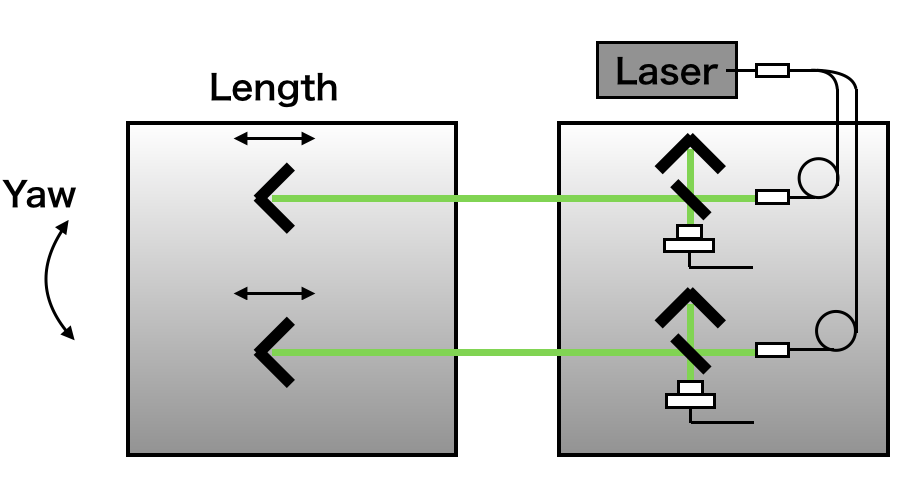
\includegraphics[width=9cm]{./img_chap5/img508a.png}
%%     \caption{Active baseline seismic isolation system using Michelson Type SPI \cite{Numata2008interferometric}. 2つのSPIで基線方向とYaw方向の制御をしている。それぞれのSPIはエンド鏡にコーナーキューブを使用している非対称マイケルソン干渉計であり、干渉信号はホモダイン検波で取得している\cite{araya2002iodine}。コーナーキューブは干渉させるためのアラインメント調整を必要としないが、その反面、角度変化と基線変化を区別できないので、SPIが2台必要になる。} \label{img:img508a}
%%   \end{center}
%% \end{figure}
To resolve the narrow linear range of the Fabry-Perot type SPI, a proto type of the Michelson type SPI was developed \cite{Numata2008interferometric}. The interferometer configuration of this proto type was the same as the GIF interferometer, and the signal detecton also the same. Thus, the type had the wide dynamic range wihout alignment control to keep the operation of the SPI. The proto type demonstrate the vibration supression of 2m baseline over several hours.

\subsection{Limitation due to CMRR}\label{sec532}
\begin{figure}[h]
  \begin{minipage}[t]{0.5\hsize}
    \centering
    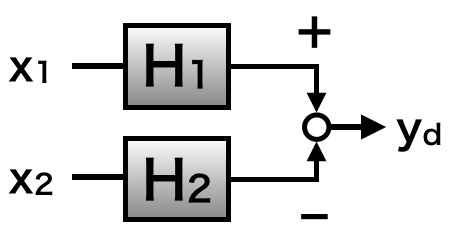
\includegraphics[width=6cm]{./img_chap5/img510a.png}
    \subcaption{two ground motion inputs ($x_1$ and $x_2$) one differential baseline change output ($y_{\mathrm{d}}$)} \label{img:img510a}
  \end{minipage}
  \begin{minipage}[t]{0.5\hsize}
    \centering
    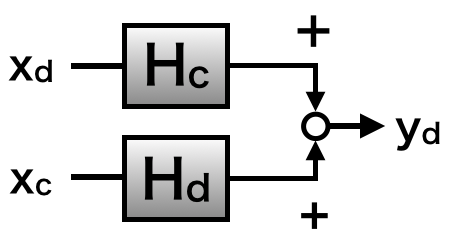
\includegraphics[width=6cm]{./img_chap5/img510b.png}
    \subcaption{two differential and common ground motion inputs ($x_{\mathrm{d}}$ and $x_{\mathrm{c}}$) one differential baseline change output ($y_{\mathrm{d}}$)} \label{img:img510b}
  \end{minipage}
  \caption{comparison of two representations.}
\end{figure}

While the active inertial seismic isolation described in the section \cref{sec:512}, the active baseline seismic isolation cannot isolate the common motion. Thus, if worse common mode rejection (CMR) of the suspensions, the common ground motion couples to the differential ground motion, which is the baseline length changes.


Consider the differential motion of the platform stages. As shown in Figure \ref{img:img510a}, the motion can be represented as 
\begin{eqnarray}
  y_{\mathrm{d}} = H_1x_1-H_2x_2 \label{eq:eq517},
\end{eqnarray}
where $x_{i},\,y_{d}$ and $H_{i}$ denote the ground motion, the stage motion, and the mechhanical transferfunction from the ground motion to the stage motion, respectively. The indicies of $i$ run in 1 or 2, which denote the name of the stages. Here, we define the differential and common motion of the ground and transferfunction as 
\begin{eqnarray} \label{eq:eq517_b}
  x_{\mathrm{d}} = {x_1-x_2},\ x_{\mathrm{c}} = {x_1+x_2}  \\
  H_{\mathrm{d}} = \frac{H_1-H_2}{2},\ H_{\mathrm{c}} = \frac{H_1+H_2}{2} \label{eq:eq517_a}.
\end{eqnarray}
The Eq(\ref{eq:eq517}) can be represented as 
\begin{eqnarray}
  y_{\mathrm{d}} &=& H_1x_1-H_2x_2 \\
  &=& H_{\mathrm{c}}x_{\mathrm{d}} + H_{\mathrm{d}}x_{\mathrm{c}}\label{eq:eq516}.
\end{eqnarray}
The last equation can be represented as shown in Figure \ref{img:img510b}. Moreover, if we define the CDMRR of this system as
\begin{eqnarray}
  H_{\mathrm{CMRR}} \equiv \frac{H_1+H_2}{H_1-H_2}=\frac{H_{\mathrm{c}}}{H_{\mathrm{d}}} \label{eq:eq519},
\end{eqnarray}
the differential system can be written as 
\begin{eqnarray}
  y_{\mathrm{d}} = H_{\mathrm{c}}\left( x_{\mathrm{d}} + \frac{1}{H_{\mathrm{CMRR}}}x_{\mathrm{c}}\right) \label{eq:eq518}
\end{eqnarray}
Eq.(\ref{eq:eq518}) indicates that increaseing the CMRR, the coupling from the common ground motion to the differential stage motion. In other words, the inverse of the CMRR is the coupling coefficient.

According to the definition of The CMRR, this factor is sensitive to the differential of two mechanical response. Thus, if the eigenfrequecy of each pendulum, the CMRR is worse above the frequency. For example, assume that the mechanical response of the stage is the single pendulum, which transfer function from the ground to stage can be given by Eq.(\ref{eq:eq502}). In the high frequency, above the eigen frequency, the response can be approximate as $H\sim{({f_0}/{f})^2}$. In this frequency region, if the eigen frequency shifts by $\Delta{f_0}$, the gain of the response differs by $2f_0\Delta{f_0}$. This amount worse the CMRR, and the common motion contaminates the differential motion.


\subsection{RMS Reduction}
The reduction of Root-mean-square (RMS) of the differential stage motion is expected by utilizing the SPI on the active seismic isolation system. Because the SPI has a good sensitivity in low-frequency including the microseisms and earth tides, the RMS of the differential stage motion can be reduced.

The reduction has some advantage for GW detectors.

\subsubsection{Improvement of Actuator Noise}
The RMS reduction of the differential stage motion can relax the requirement of the actuator on the test mass. The actuator on the test mass can only actuate weak force because the strong actuator would introduce the actuation noise to the sensitivity \cite{michimura2017mirror}. Therefore, the RMS reduction on the top stage can reduce the load on the test mass actuators. This means the improvement of the test mass actuator's noise directly, moreoever, means that the actuator's dynamic range can be became wider.

\subsubsection{Improvement of Glitch Noise}
The reduction of the test mass actuator's load reduce the glicth noise such as the Barkhausen noise. This noise is caused by the large DC voltage on the test mass actuators and actuators above the test mass \cite{aasi2015characterization}.




\section{Baseline Compensation System}\label{sec:52}
The baseline compensation system is the active baseline seismic isolation syste ugin the GIF. 

\subsection{Purpose}
The purpose of the baseline compensation system is to reduce the RMS of the cavity length fluctuation from 1 Hz to DC. In this region, the RMS motion in cavity length is mainly disturbed by the seismic noise such as the microseisms ($\sim 200\,\mathrm{mHz}$), large earthquake in distant place ($< 100\,\mathrm{mHz}$), air pressure response ($< 20\, \mathrm{mHz}$), and earth tides ($\sim 10^{-5}\,\mathrm{Hz}$). Moreover, the RMS of these seismic motion is comparable with several $1\sim100\,\mathrm{um}$, which is much greter than the test mass actuator's range. Therefore, the compensation of the cavity length disturbed by these seismic noise not only the improve stability of the detector operation but also the reduce the glitch noises in GW signal.

\subsection{Concept}


Below 1 Hz, the displacement of the 3000 m baseline is given by 2 times of that of the 1500 m baseline.

\begin{figure}[h]
  \begin{center}   
    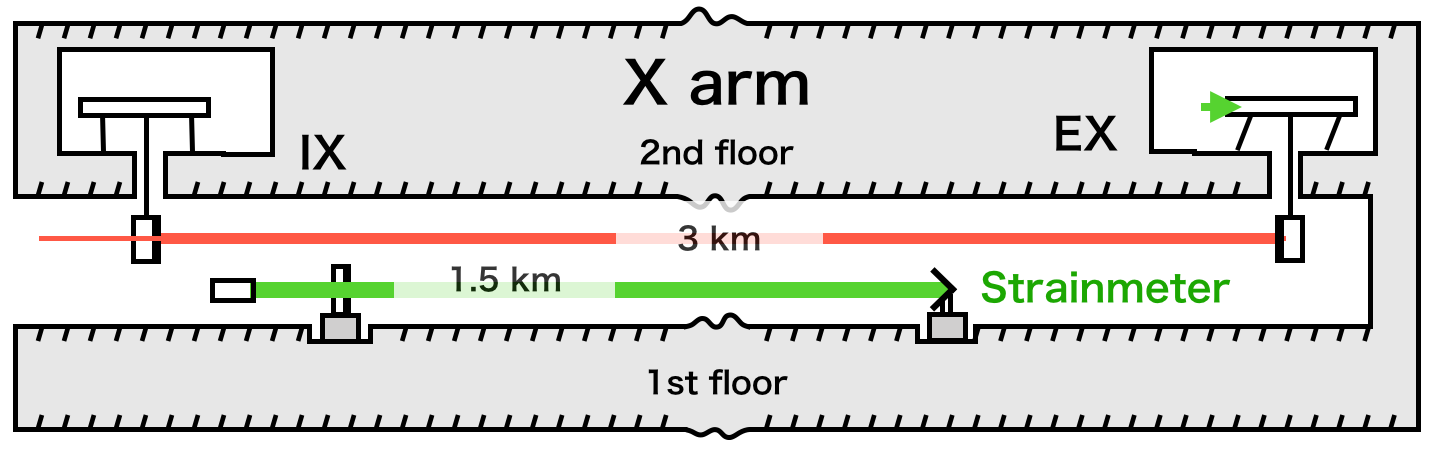
\includegraphics[width=14cm]{./img_chap5/img512.png}
    \caption{} \label{img:img512}
  \end{center}
\end{figure}



\subsection{GIF as a SPI}


\subsection{Control methods}
\begin{figure}[h]
  \begin{center}   
    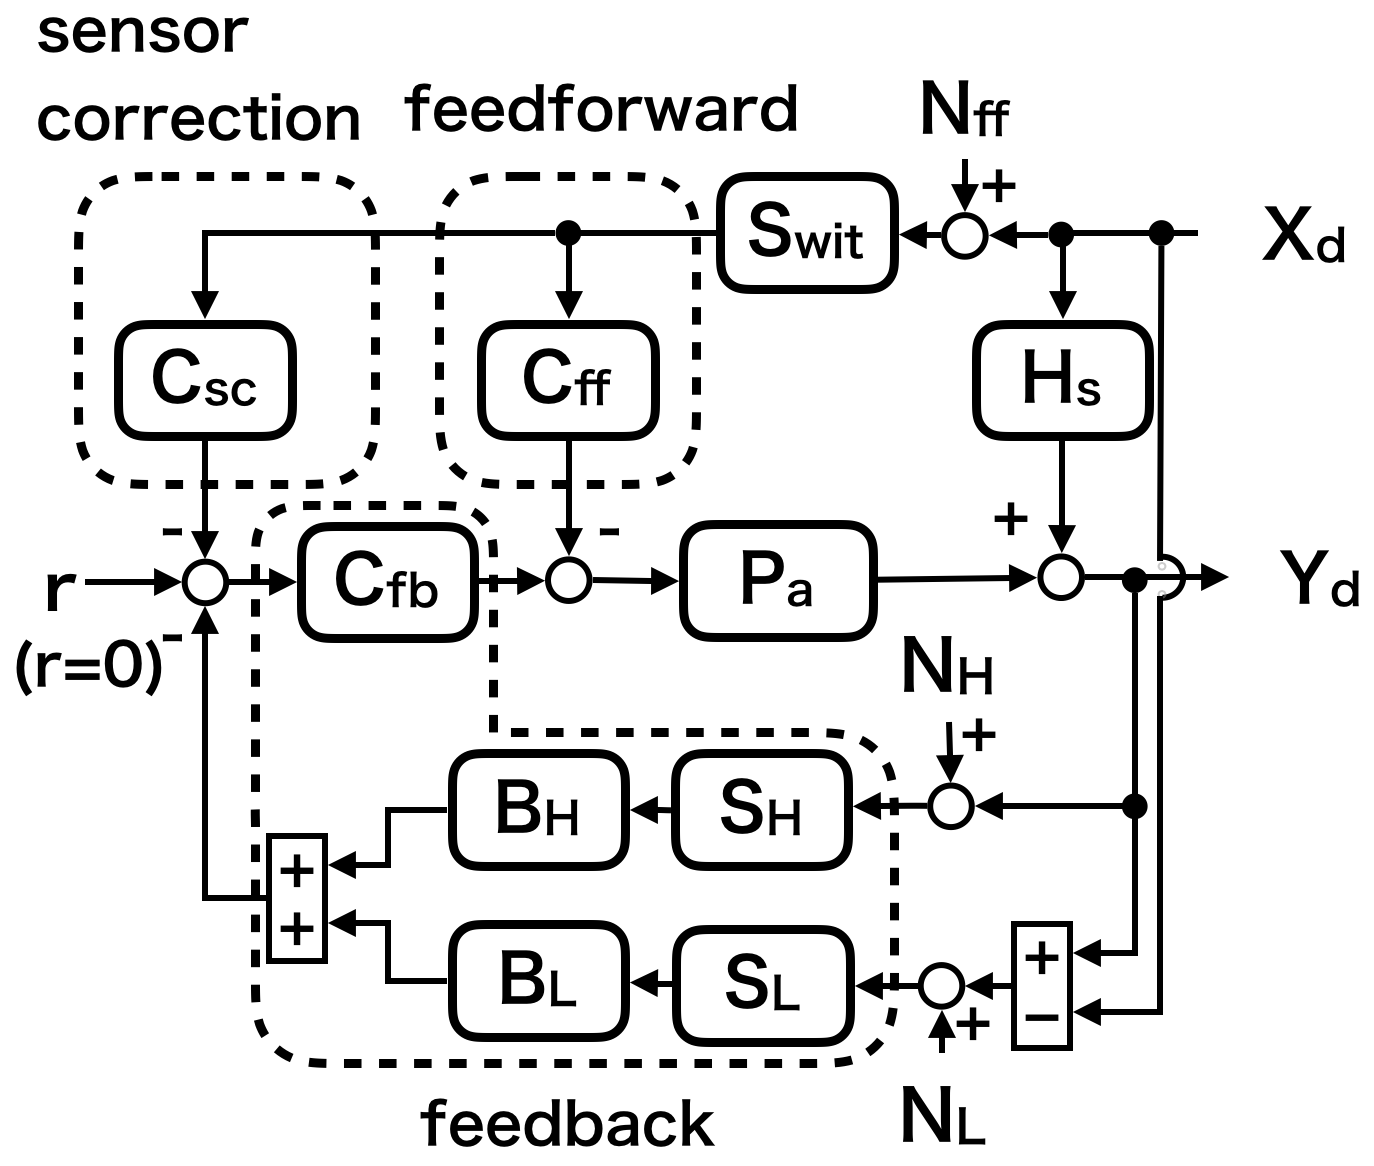
\includegraphics[width=10cm]{./img_chap5/img511.png}
    \caption{The block diagram of the active baseline seismic isolation system.} \label{img:img511}
  \end{center}
\end{figure}

In this section, we describe the control method of the active baseline seismic isolation system using the SPI interferometer. According to the previous section \cref{sec532}, the differential output can be represented as the differential and common inputs. This diagram is the same as the Figure \ref{img:img503} except the input ground motion and output stage motion as shown in Figure \ref{img:img511}. In this diagram, the common component of the ground motions are ignored because of assuming the large CMRR. It that means also that the common transfer function is equal to the single one, according to Eq.(\ref{eq:eq517_a}).

The displacement of the differential motion of the stages is given by 
\begin{eqnarray}\nonumber
  Y_{\mathrm{d}} &=&\frac{G}{1+G}L\Delta_{\mathrm{sc}} X_{\mathrm{d}} + \frac{1}{1+G} \Delta_{\mathrm{ff}} X_{\mathrm{d}}\\ \nonumber
  &+& \frac{G}{1+G}\left(HN_{H}+LN_{L}\right) + \frac{G}{1+G}C_{\mathrm{sc}}S_{\mathrm{wit}}N_{\mathrm{ff}} \\ 
  &+& \frac{1}{1+G}P_{\mathrm{a}} C_{\mathrm{ff}}S_{\mathrm{wit}}N_{\mathrm{ff}} \label{eq:eq520},
\end{eqnarray}
where $X_{\mathrm{d}}$ and $Y_{\mathrm{d}}$ are the differential ground motion and stage motion, respectively, and other terms are the same as Eq.(\ref{eq:eq518}).




\section{Summary of the Chapter}
 % Arm Length Compensation for Global Seismic Control
\chapter{Demonstration of Arm Length Compensation Control}
\section{Experimental Arrangement}
Xアーム共振器をつかって評価した。
\subsection{...}
\section{Results}
\subsection{...}
\section{Discussion and Summary of the Chapter}
\subsection{Discussion}
\subsection{Summary}
 % Demonstration of Arm Length Compensation
\chapter{Conculusion and Future Directions}
\section{Conclusion}
\section{Future Directions}
 % Conculusion and Future Directions
\appendix
\chapter{KAGRA}
\section{Overview of KAGRA}
\subsection{Status of KAGRA}
KAGRA is a 3km laser interferometer constructed in Kamioka, Gifu, Japan, and is now in its final commissioning phase. KAGRA is now commissioning to observe with LIGO and Virgo in the third observation (O3), through the two test operation phase. The phases of the KAGRA project are listed in Table \ref{tb:tb600}. The first test operation named initial KAGRA (iKAGRA), which is taken place from March to April 2016, was a demonstration of the 3-km Michelson interferometer. In this operation, While the test masses are not in cryogenic temperature but room temperature, KAGRA demonstrates the operation of the km-scale interferometer in the underground. Next, the second test operation named baseline KAGRA (bKAGRA) demonstrated the cryogenic Michelson interferometer from April to May 2018. Although this interferometer was not for sensitivity enhanced configuration, the cryogenic operation, which is the key feature of KAGRA, could be demonstrated. Now, in December 2019, KAGRA is faced with the O3 observation with the Michelson interferometer, whose each arm has Fabry-Perot optical cavities (FPMI). To join the O3, KAGRA is now tunning the interferometer operation and hunting the several technical noises.
\begin{table}[h]
  \caption{Summary of the phases of KAGRA. MI: Michelson Interferometer, FPMI: Fabry-Perot Michelson Interferometer, DRFPMI: Dual-Recycled Fabry-Perot Michelson Interferometer, RSE: resonant sideband extraction}
  \begin{tabular}{lllll}
    \toprule
    &iKAGRA& \begin{tabular}{l}bKAGRA\\Phase1\end{tabular} & \begin{tabular}{l}bKAGRA\\for O3\end{tabular}  & \begin{tabular}{l}bKAGRA\\(final)\end{tabular}  \\ \midrule
        
        \begin{tabular}{l}Year\end{tabular}& \begin{tabular}{l}2016\\Mar - Apr\end{tabular}&\begin{tabular}{l}2018\\Apr - May\end{tabular} & \begin{tabular}{l}2019\\Dec - \end{tabular} & \begin{tabular}{l}2020 -\\(planned)\end{tabular} \\
              \begin{tabular}{l}Configuration\end{tabular} & \begin{tabular}{l}MI\end{tabular} & \begin{tabular}{l}MI\end{tabular} & \begin{tabular}{l}FPMI\end{tabular} & \begin{tabular}{l}DRFPMI\\(RSE)\end{tabular}\\
                      
                      \begin{tabular}{l}Test mass\\temperature\end{tabular} & \begin{tabular}{l}room temp.\end{tabular}& \begin{tabular}{l}18K\\room temp.\end{tabular} & \begin{tabular}{l}18K\\room temp.\end{tabular}  & \begin{tabular}{l}22K\end{tabular}             \\ \bottomrule
  \end{tabular}
\end{table}

%% KAGRAの最終的な感度は、resonant sideband extraction technique をもちいた Dual-Recycled Fabry-Perot Michelson interferometer で達成される。KAGRAの設計感度をFig.\ref{img:img600}に示す。

%% \begin{figure}[h]
%%   \begin{center}   
%%     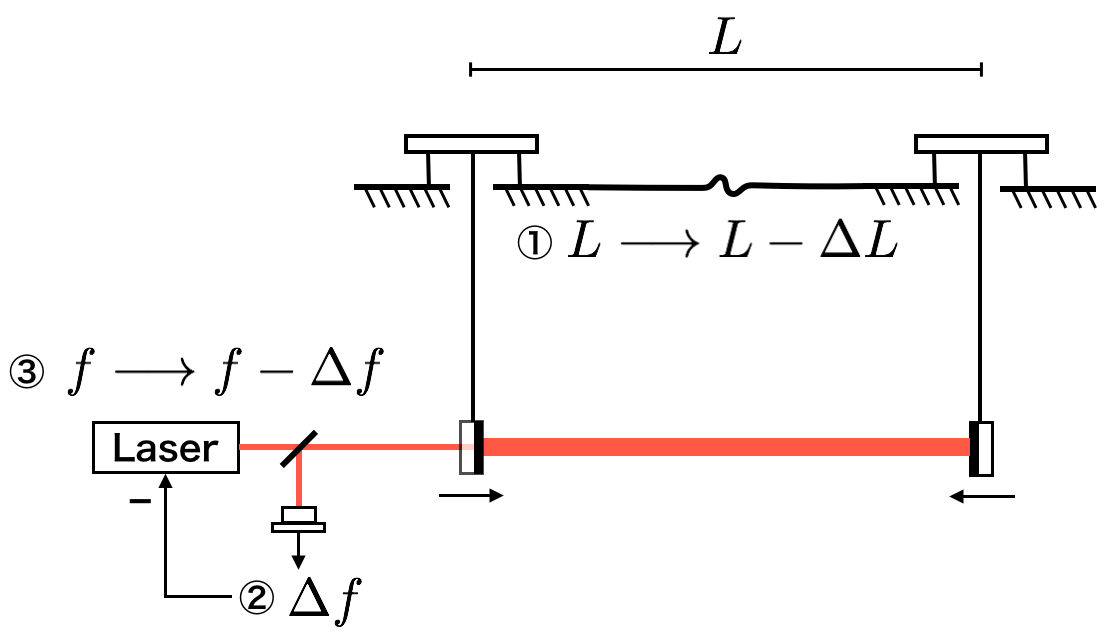
\includegraphics[width=12cm]{./img_chap6/img600.png}
%%     \caption{The designed sensitivity of KAAGRA \cite{akutsu2019first}}{}\label{img:img600}
%%   \end{center}
%% \end{figure}

\subsection{Main Interferometer}
The main interferometer of KAGRA is shown in Figure \ref{img:img601}. The interferometer configuration of KAGRA is also the same as other GW detectors such as advanced LIGO and advanced Virgo, the Michelson interferometer with Fabry-Perot optical cavity on each arm and two recycling optical cavities. The different feature of these detectors is the cryogenic test masses. To cool down to cryogenic, typically 22 K, the test mass mirror is made of sapphire because of the high thermal conductivity and mechanical Q value even in a cryogenic environment. These properties can reduce some problems of the interferometric GW detectors; thermal lens effect and thermal noise.
\begin{figure}[p]
  \begin{minipage}{15cm}
    \begin{center}   
      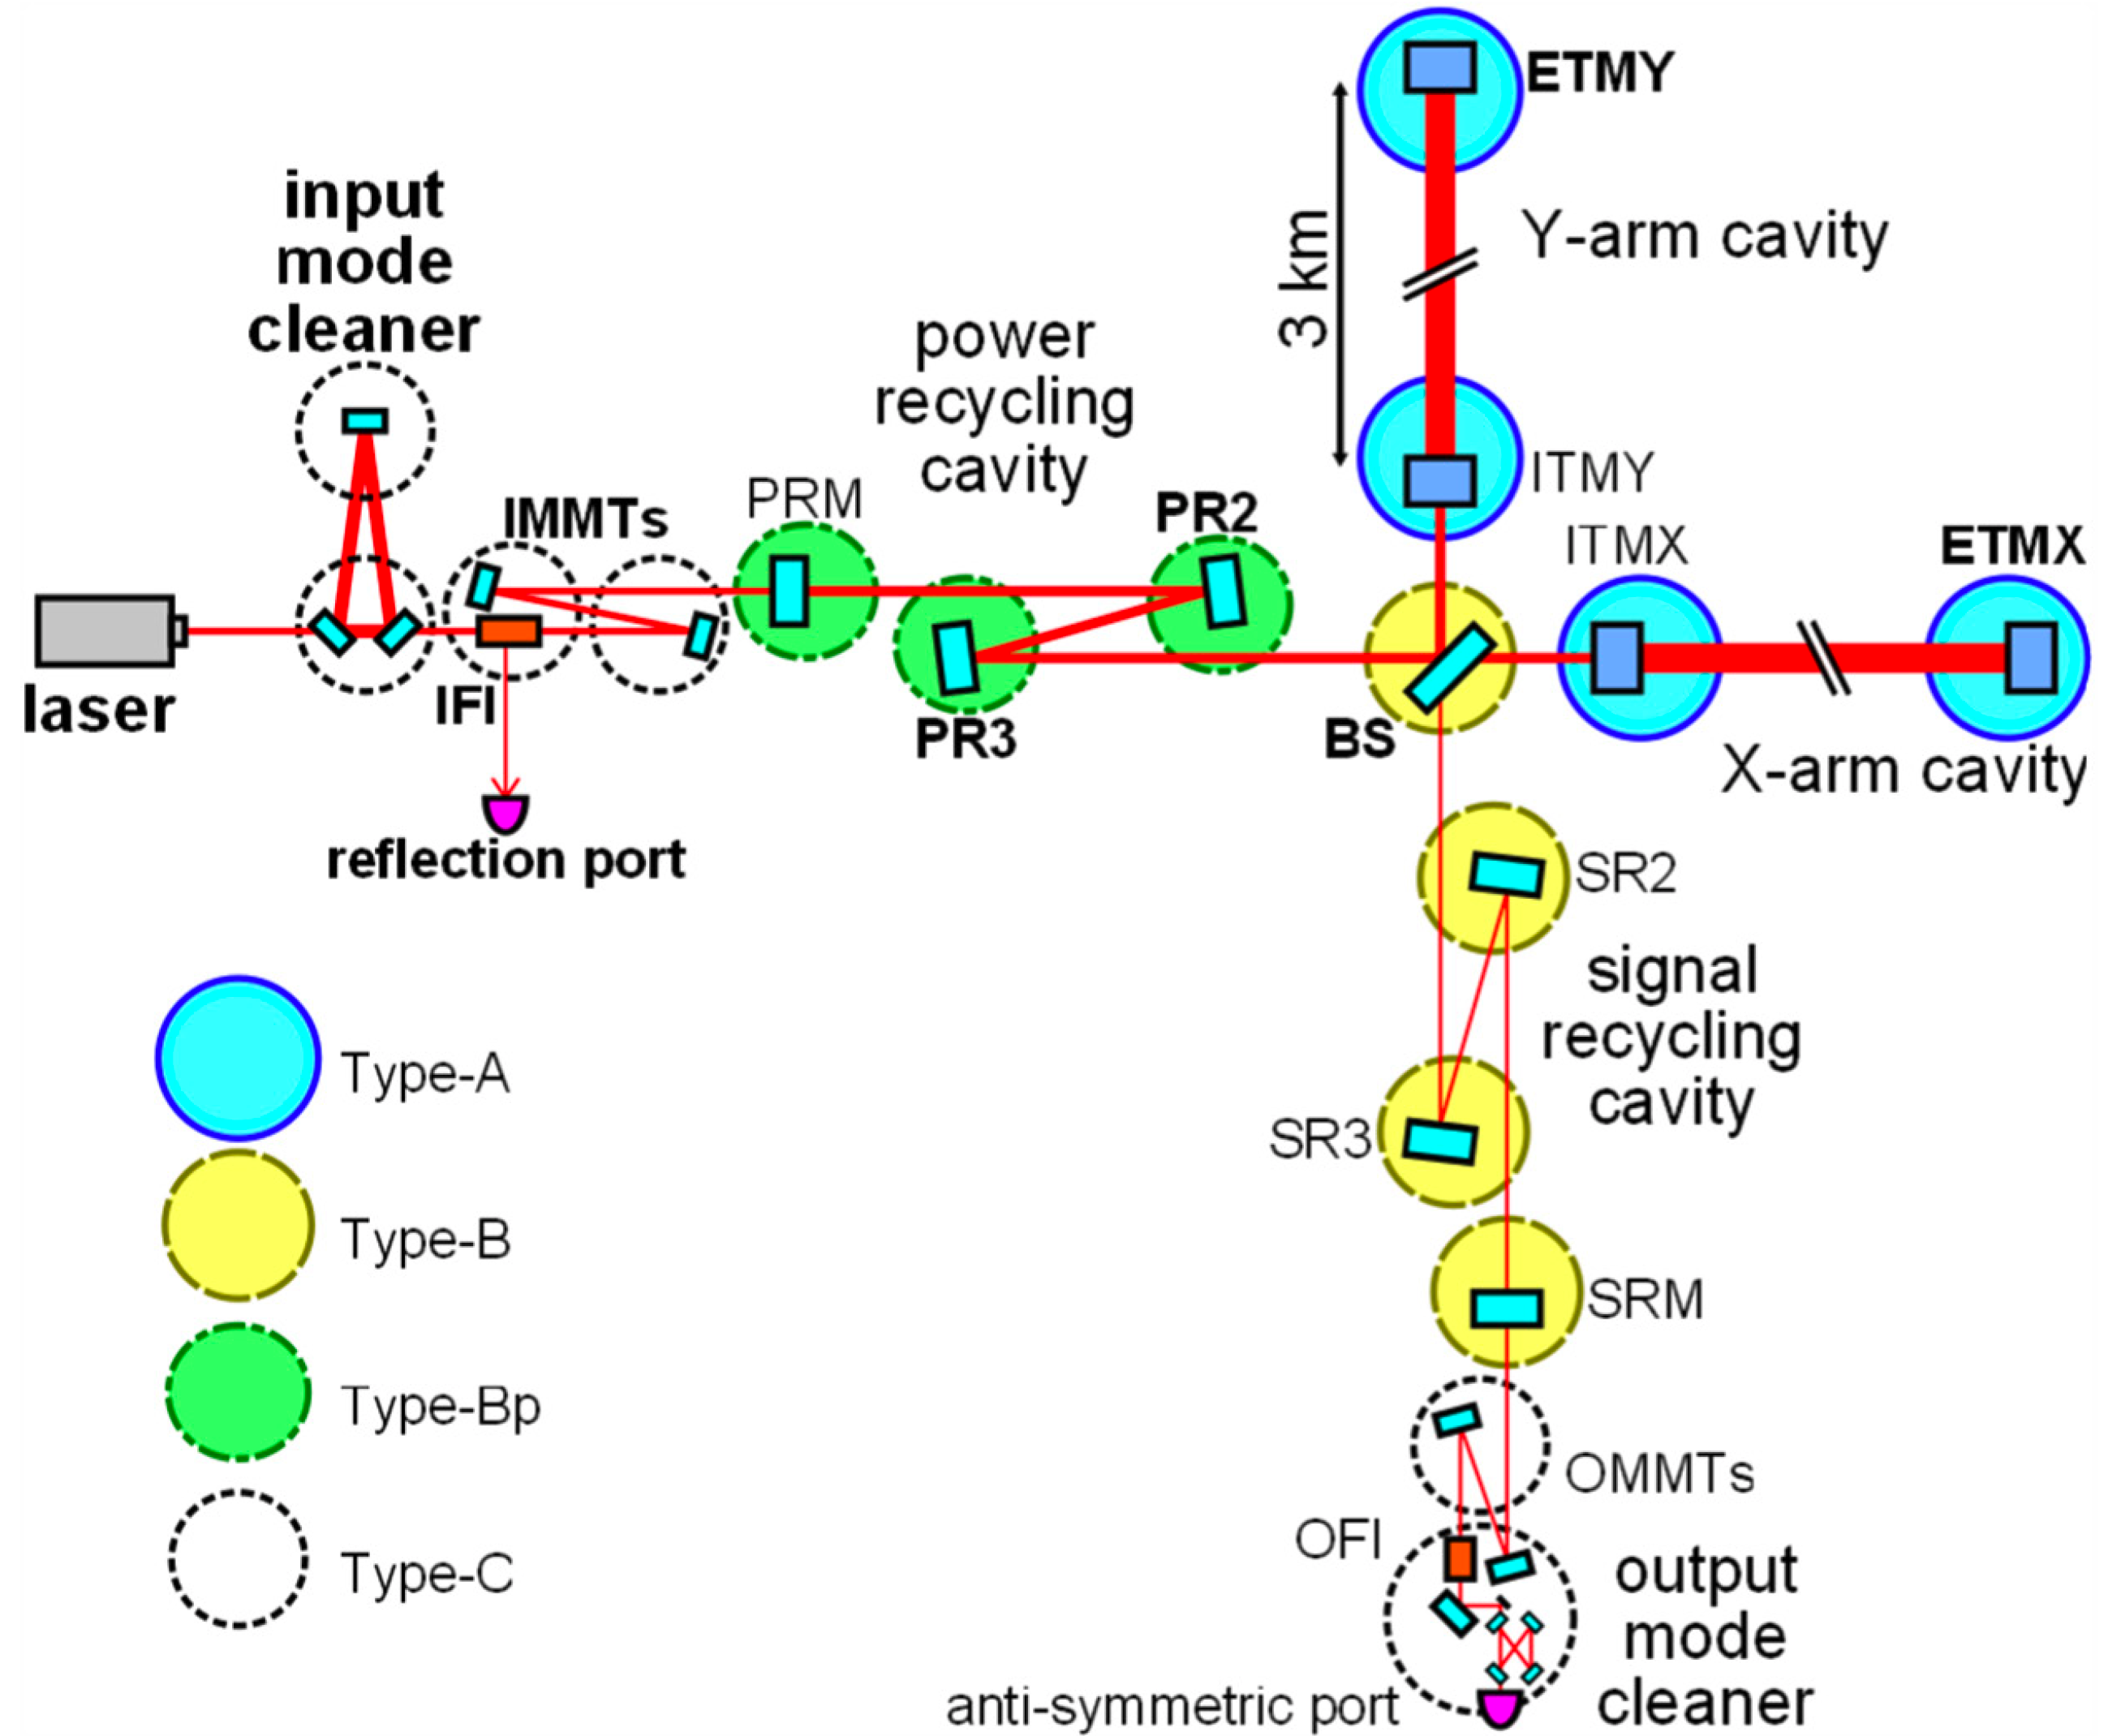
\includegraphics[width=13cm]{./img_chap6/img601.png}
      \subcaption{Schematic interferometer configuration of KAGRA \cite{akutsu2019first}}{}\label{img:img601} \hfill\vspace{10pt}
    \end{center}
  \end{minipage}
  \begin{minipage}{15cm}
    \begin{center}   
      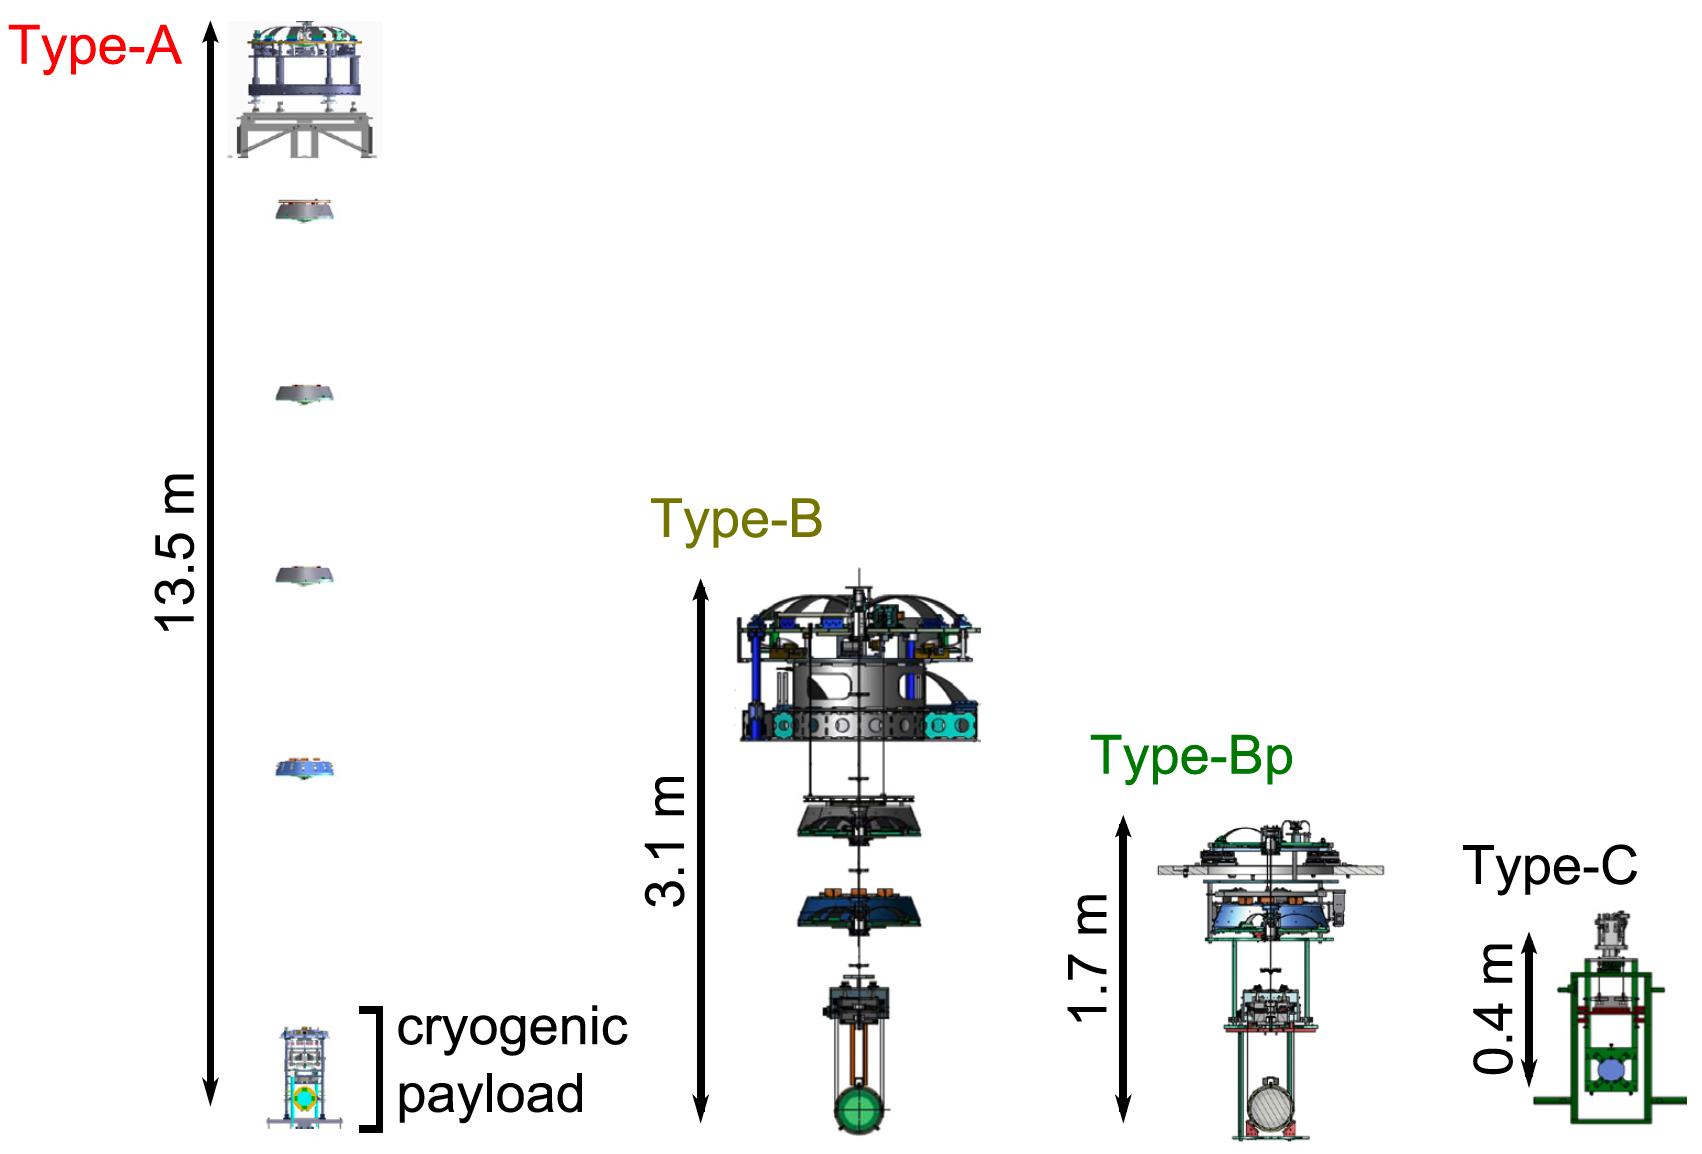
\includegraphics[width=13cm]{./img_chap6/img601b.png}
      \subcaption{KAGRA mirror suspension system \cite{akutsu2019first}}\label{img:img601b}
    \end{center}
  \end{minipage}
  \caption{Interferometer configuration and mirror suspension system}{}
\end{figure}
The main interferometer is divided into four parts; (1) arm cavities, (2) input and output mode cleaners (IMC and OMC), (3) power recycling cavities (PRC), (4) and signal recycling cavities (SRC). The first, the arm cavities are composed of input test masses (ITMs) and end test masses (ETMs) with high reflectivity corresponding to a finesse of 1530 not to increase the internal cavity power. The second, while IMC is used for clean out the higher-order spatial mode and stabilizing the frequency of the main input laser, OMC is used for clean out the unwanted higher-order spatial modes and frequency sideband of the output beam. The IMC is the triangle optical cavity which is made to stabilize the input laser frequency above 1 Hz. The OMC is the bow-tie cavity composed of four mirrors. The third, PRC is used for increasing the input laser power by ten times. This cavity is composed of three mirrors named PRM, PR2, and PR3, respectively. The forth, SRC is used to expand the bandwidth of GW signals. This technique is more important than Advanced LIGO and Advanced Virgo because the bandwidth is narrower than other detectors due to a high finesse arm cavity of KAGRA. 

\subsection{Mirror Suspension System}
All mirrors of the interferometer are suspended by four types of suspensions: Type-A, Type-B, Type-Bp, Type-C. These suspensions are shown in Figure \ref{img:img601b}. The Type-A is a 13.5 m scale 9-stage pendulum suspending the test mass mirror. The Type-B is a small size of Type-A suspension for suspending the signal recycling mirrors and beam splitter mirror. The Type-Bp is also a small size of Type-B but without the pre-isolator stage, which is for the power recycling mirrors. The type-C is the simple 2-stage suspension used in TAMA300 but with minor modification.
\begin{figure}[p]
  \begin{center}   
    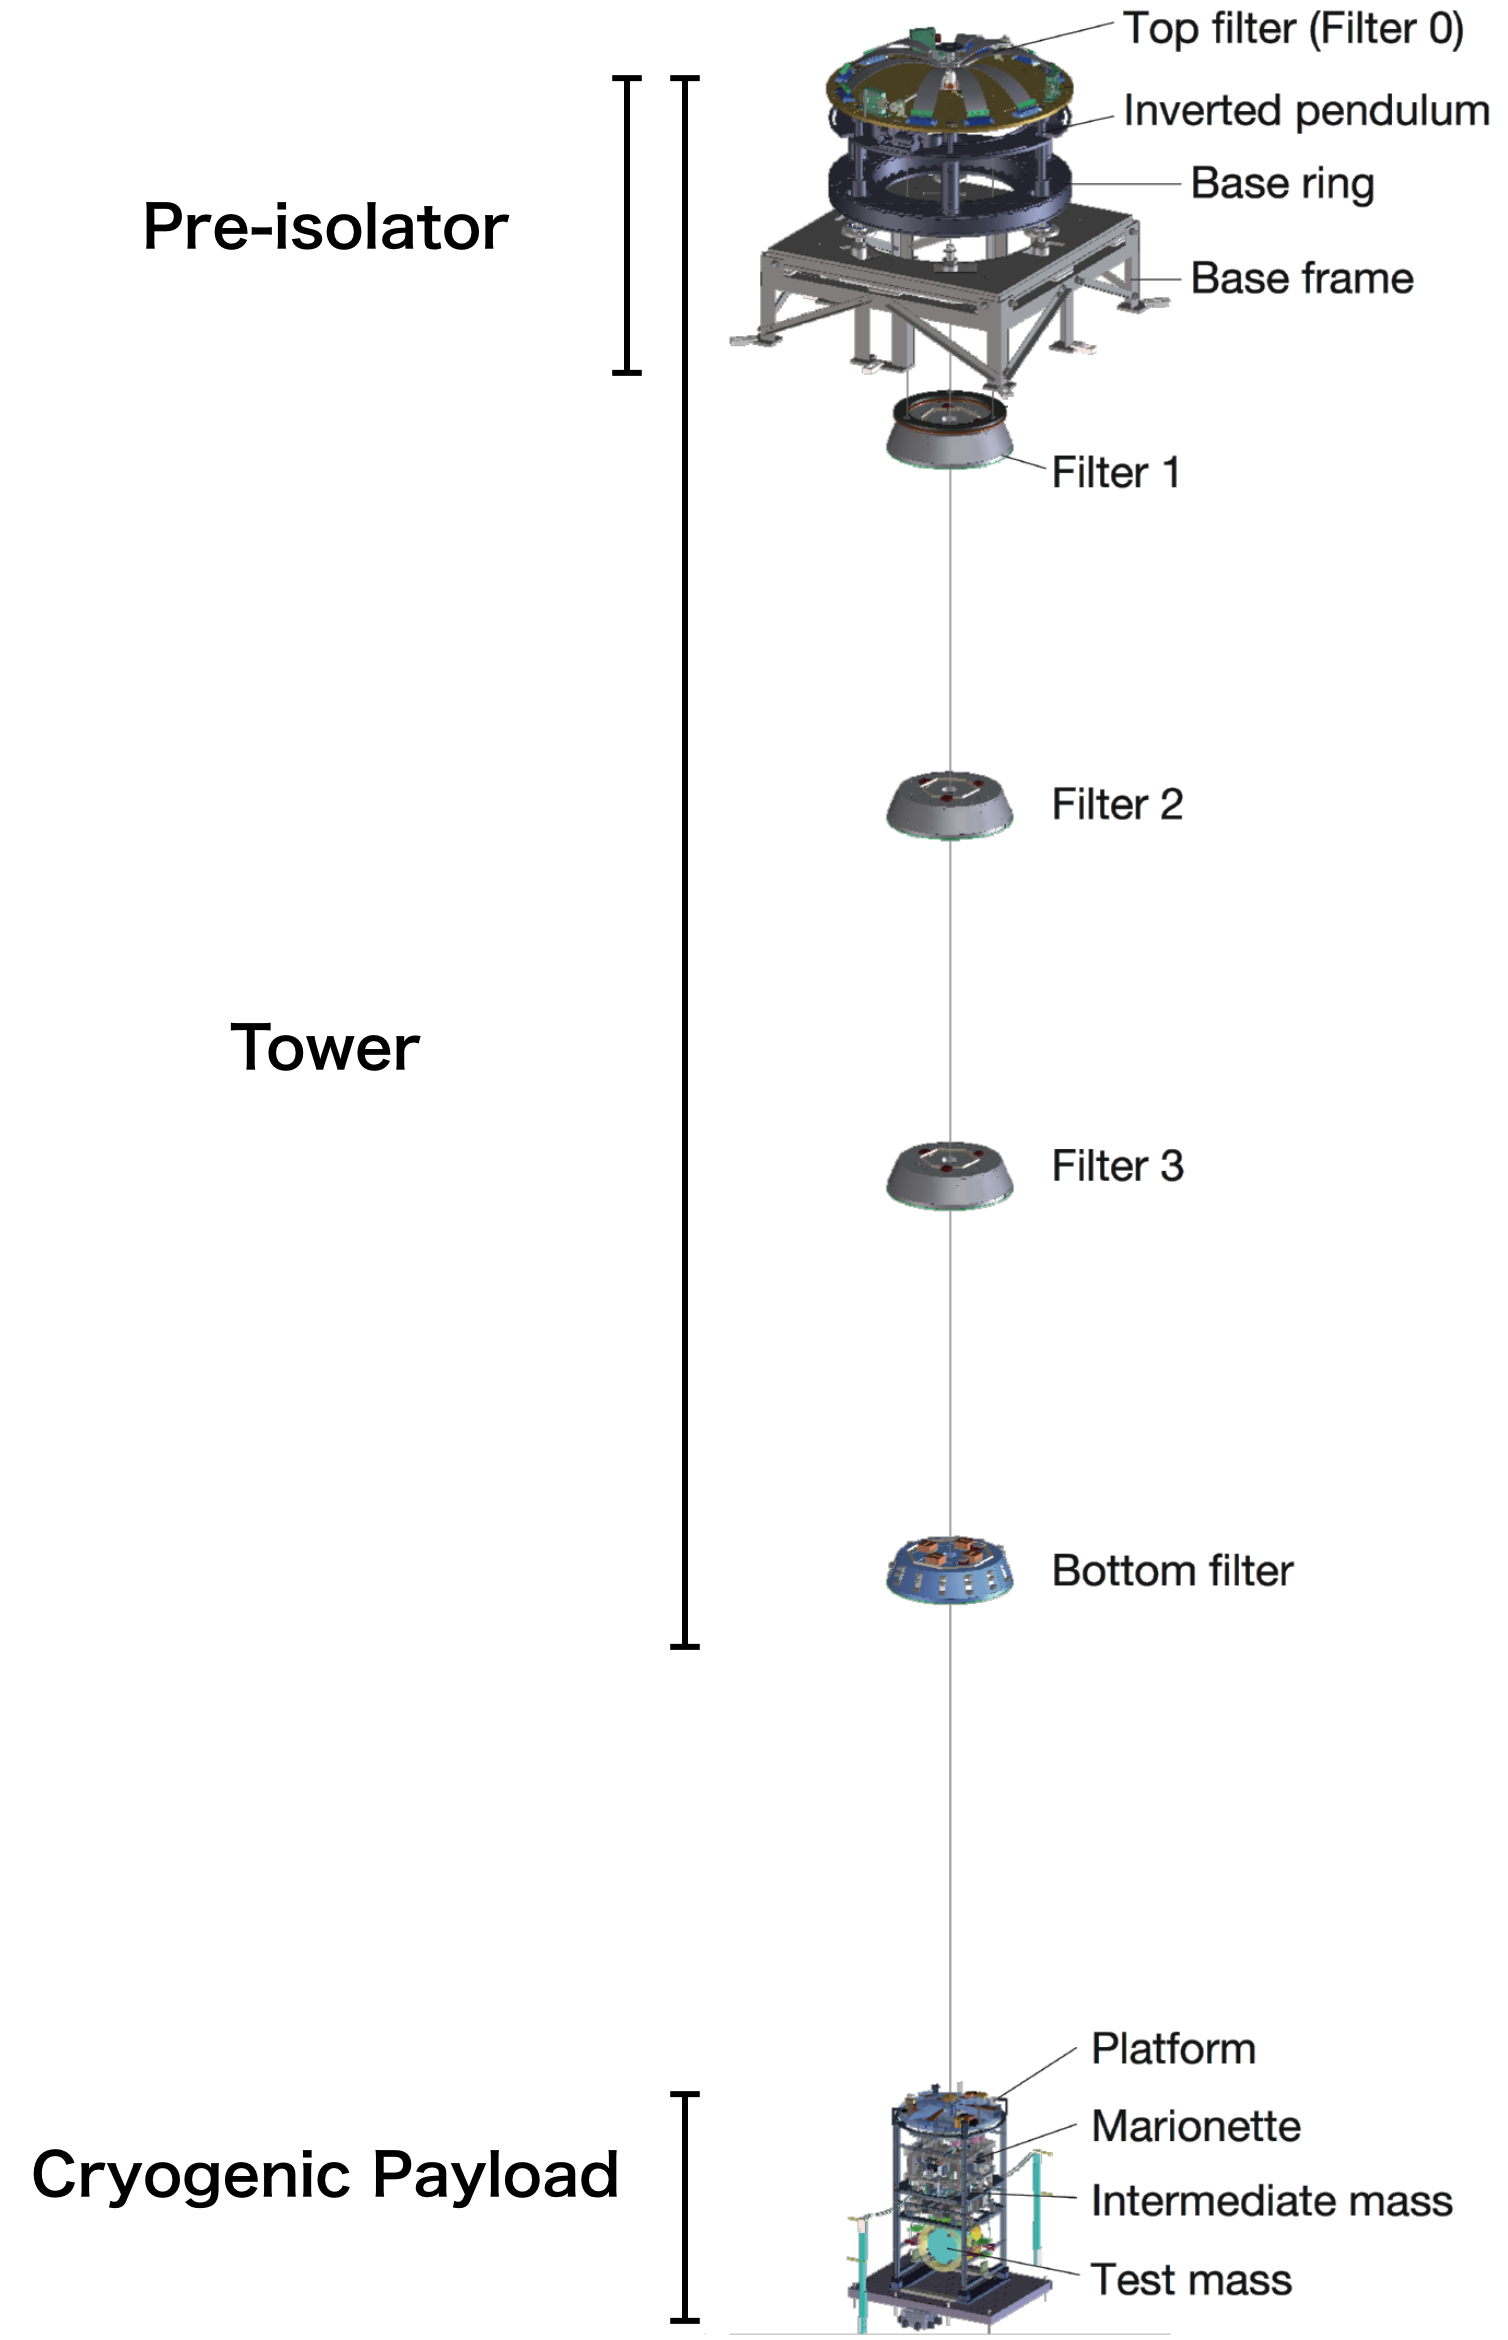
\includegraphics[width=13cm]{./img_chap6/img604.png}
    \caption{An overview of the Type-A suspension \cite{Okutomi2019development}. Test mass is suspended by a $13.5\,\mathrm{m}$ pendulum consisted of several mechanical filters. The suspension point of the long pendulum is supported by the pre-isolator, which consists of an inverted pendulum, on the ground through the base frame and base ring.}\label{img:img604}
  \end{center}
\end{figure}

\begin{figure}[p]
  \begin{minipage}{1.0\hsize}
    \begin{center}   
      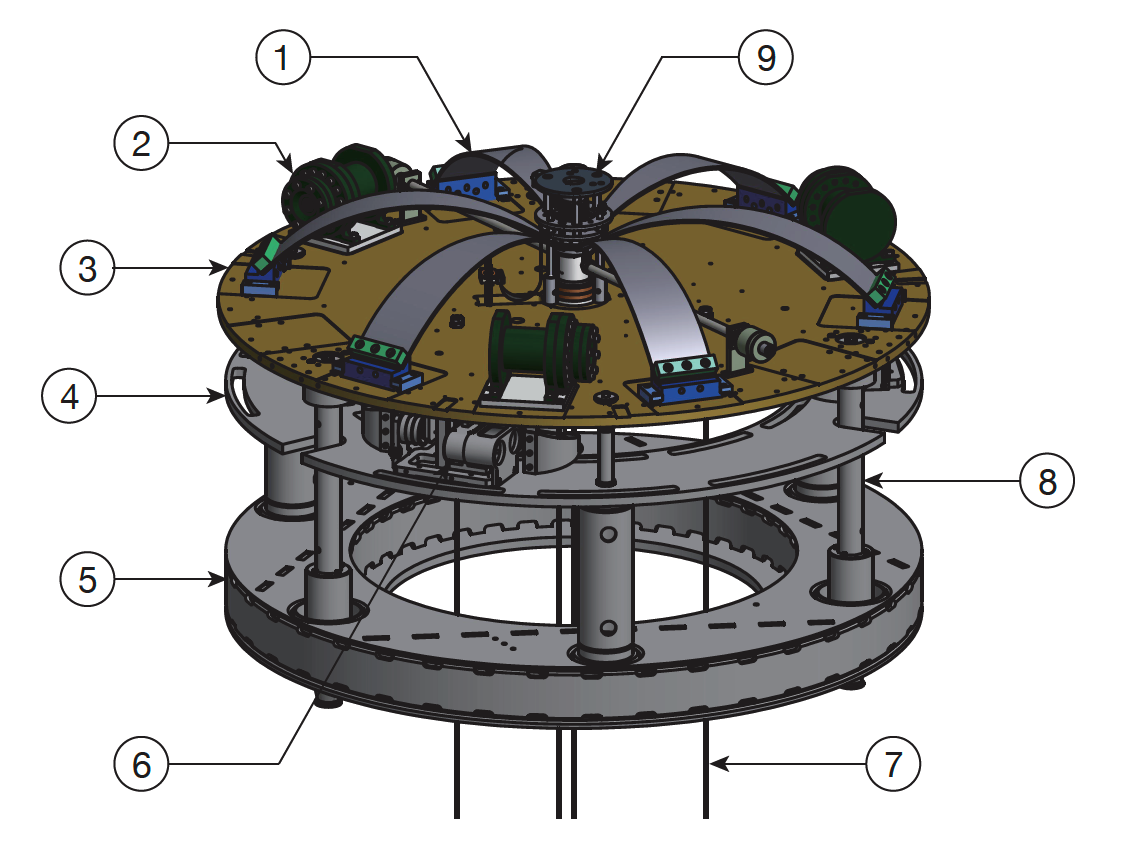
\includegraphics[width=12cm]{./img_chap6/img603a.png}
      \subcaption{Pre-isolator stage (PI). (1) Cantilever blade for GAS. (2) Geophone (3) Table of the top stage (4) Refernce frame rigidly connected to the base ring (5) The base ring mounted on the ground (6) LVDT and the coil magnet actuator (7) suspension wire to suspend the lower stages (8) leg of the inverted pendulum (IP). Figure is cited from figure 3.9 in \cite{Okutomi2019development}}\label{img:img603a}
    \end{center}
  \end{minipage}\\   
  \begin{minipage}[b]{0.5\hsize}
    \begin{center}
      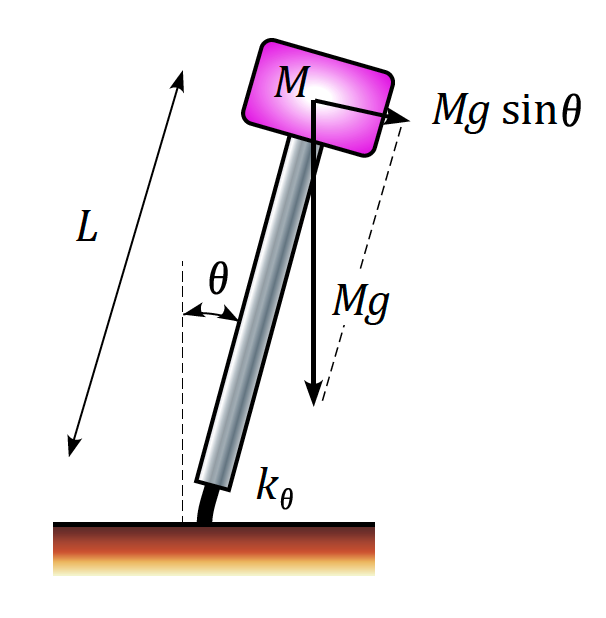
\includegraphics[width=8cm]{./img_chap6/img603b.png}
      \subcaption{Leg of the inverted pendulum (IP) \cite{sekiguchi2016astudy}.}\label{img:img603b}
    \end{center}
  \end{minipage}
  \begin{minipage}[b]{0.5\hsize}
    \begin{center}
      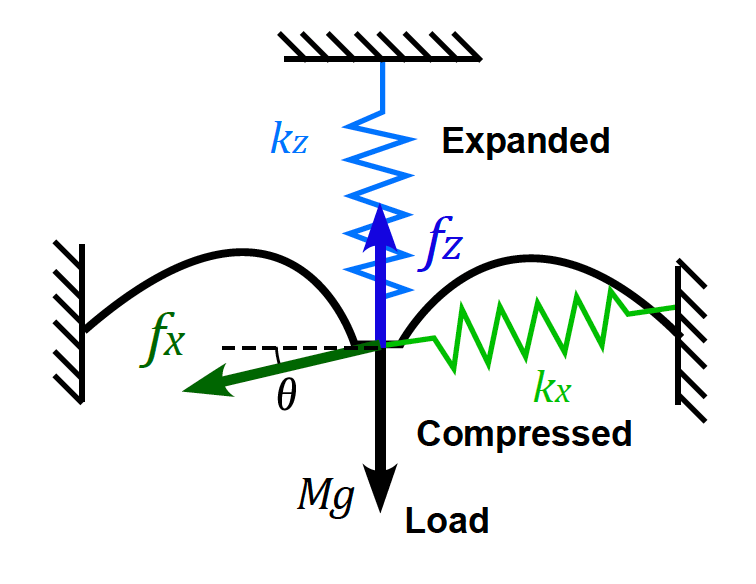
\includegraphics[width=8cm]{./img_chap6/img603c.png}
      \subcaption{Geometrical Anti-Spring \cite{sekiguchi2016astudy}.}\label{img:img603b}
    \end{center}
  \end{minipage}  
  \caption{CAD drawing of the pre-isolator (top) and main mechanical components of PI; IP leg and GAS (bottom).}
\end{figure}


\section{KAGRA Type-A Suspension}
\subsection{Overview}
In order to suspend the cryogenic test mass, as shown in Fig.\ref{img:img604}, KAGRA Type-A suspension has two parts; cryogenic payload and $13.5\,\mathrm{m}$ room temperature tower pendulum \cite{Okutomi2019development}. The cryogenic payload consists of Platform, Marionette, Intermediate mass, Test mass. The tower consists of 5 mechanical filters; Top filter, F1, F2, F3, and Bottom filter. Moreover, the suspension point of the tower is suspended by the pre-isolator stage which has an inverted pendulum.

In terms of the low-frequency seismic attenuation, the pre-isolator is the important mechanical part.



\subsection{Pre-Isolator stage (PI)}
The pre-isolator (PI) is active seismic isolation for the suspension point of the long Type-A or Type-B suspensions. As shown in Figure \ref{img:img603a}, the suspension point is on the platform stage supported by the inverted pendulum (IP) which isolates the seismic noise in a horizontal direction. For vertical direction, geometric anti-spring (GAS) suspends this point. Especially, the horizontal motion of the platform stage is isolated by using the feedback control with the inertial sensor and the relative position sensor.

\subsubsection{Inverted pendulum for horizontal vibration isolation}
Inverted pendulum (IP) is the low eigenfrequency pendulum because this mechanical filter can adjust the effective spring constant to small value by tuning the load on the platform stage. The angular eigenfrequency of the single IP leg is given by \cite{sekiguchi2016astudy}
\begin{eqnarray}
  \omega_{\mathrm{IP}}=\sqrt{\frac{g}{L}\left(\frac{k_{\mathrm{\theta}}/gL-M}{M}\right)},\\
\end{eqnarray}
where $k_{\theta}$ is the bending spring constant of the flexure, $M$ is the mass of the stage, and $L$ is the length of the leg. Although the eigenfrequency can be adjusted to zero in principle, actual eigenfrequency is designed at least 100 mHz because it is unstable when the term in the square root is minus value.

\subsubsection{Geometric Anti-Spring for vertical vibration isolation}
Geometric anti-spring is also the low eigenfrequency pendulum in a vertical direction. The eigenfrequency is adjusted to small value by compressing the cantilever blades as shown in Figure \ref{img:img603b}. The angular eigenfrequency is given by 
\begin{eqnarray}
  \omega_{\mathrm{GAS}} = \sqrt{\frac{1}{M}\left[{ k_{z}- \left(\frac{l_{0}}{x_{0}}-1\right) k_{x}}\right]},
\end{eqnarray}
where $M$ is the load mass, $k_{\mathrm{x}}$ and $k_{\mathrm{z}}$ are the elastic constant of the compressed catilevers, $l_{0}$ is a natural length of the blades, $x_0$ is the horizontal distance between the central keystone and the support poit of the blades. One can find that the angular eigenfrequency of the GAS is reduced when $x_{0}<l_{0}$.

\subsubsection{Liner Variable Differential Transducer (LVDT)}
\begin{figure}[h]
  \begin{center}   
    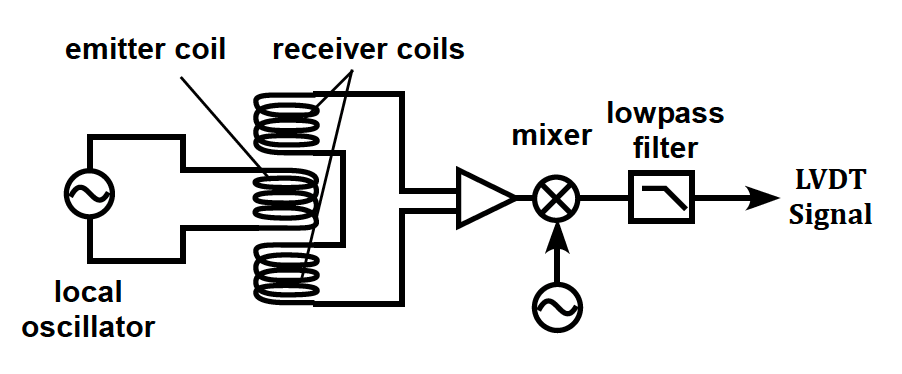
\includegraphics[width=10cm]{./img_chap6/img605.png}
    \caption{\cite{sekiguchi2016astudy}}\label{img:img605}
  \end{center}
\end{figure}
LVDT is a wide range relative position sensor composed of three coils \cite{Tariq2002hh}. shown in Fig.\ref{img:img605}. The emitter coil is mounted on the pre-isolator stage and driven with a sinusoidal signal to emit a modulated magnetic field. The two receiver coils are mounted on the reference structure, and these coils are counter-wound to each other. When the emitter coil is on the center of two receiver coils, the induced voltage is not emitted from the receiver coils. On the other hand, when the pre-isolator is moved, a sinusoidal signal appears on the receiver coils. Therefore, after demodulating this signal, the amplitude of the output signal is proportional to the displacement from the LVDT geometrical center.

\subsubsection{Coil-magnet actuator}
We use a voice-coil type wide range actuator to move the pre-isolator stage \cite{wang2002constant}.


\chapter{Gaussian Beam}
\section{Gaussian beam}
The ideal Gaussian beam has a fundamental spatial mode called $\mathrm{TEM}_{00}$. The whose electric field of the beam propagating to $z$ axis is given by \cite{bond2016interferometer,svelto1998principles}
\begin{eqnarray}
  u(x, y, z)=\sqrt{\frac{2}{\pi{w^2(z)}}} \exp \left(i\zeta(z)-\mathrm{i} k \frac{x^{2} +y^{2}}{2 R(z)}-i\frac{2\pi}{\lambda}z\right)
  \exp \left(-\frac{x^{2}+y^{2}}{w^{2}(z)}\right),  \label{eq:eq415}
\end{eqnarray}
where $\lambda,\,w_0$ are the wavelength and the beam radius at $x=0$ of the beam. In addition,
\begin{eqnarray}
  z_0 &=& \frac{\pi{w^2_0}}{\lambda} \\ \label{eq:eq415_a}
  w(z) &=& w_0\sqrt{1+\left(\frac{z}{z_0}\right)^2}, \\ \label{eq:eq415_b}
  R(z) &=& z\left[1+\left(\frac{z_0}{z}\right)^2\right],\\ \label{eq:eq415_c}
  \phi(z) &=& \arctan\left(\frac{z}{z_0}\right) \label{eq:eq415_d}
\end{eqnarray}
are Rayliegh range and radius, curvature, and Gouy phase of the beam as a function of $z$, respectively. One can find that power of the beam $|u^2|$ has a Gaussian distribution as shown in Figure  \ref{img:img415a} according to Eq.(\ref{eq:eq415}). 

\begin{figure}[p]
  \begin{minipage}{14cm}
    \centering    
    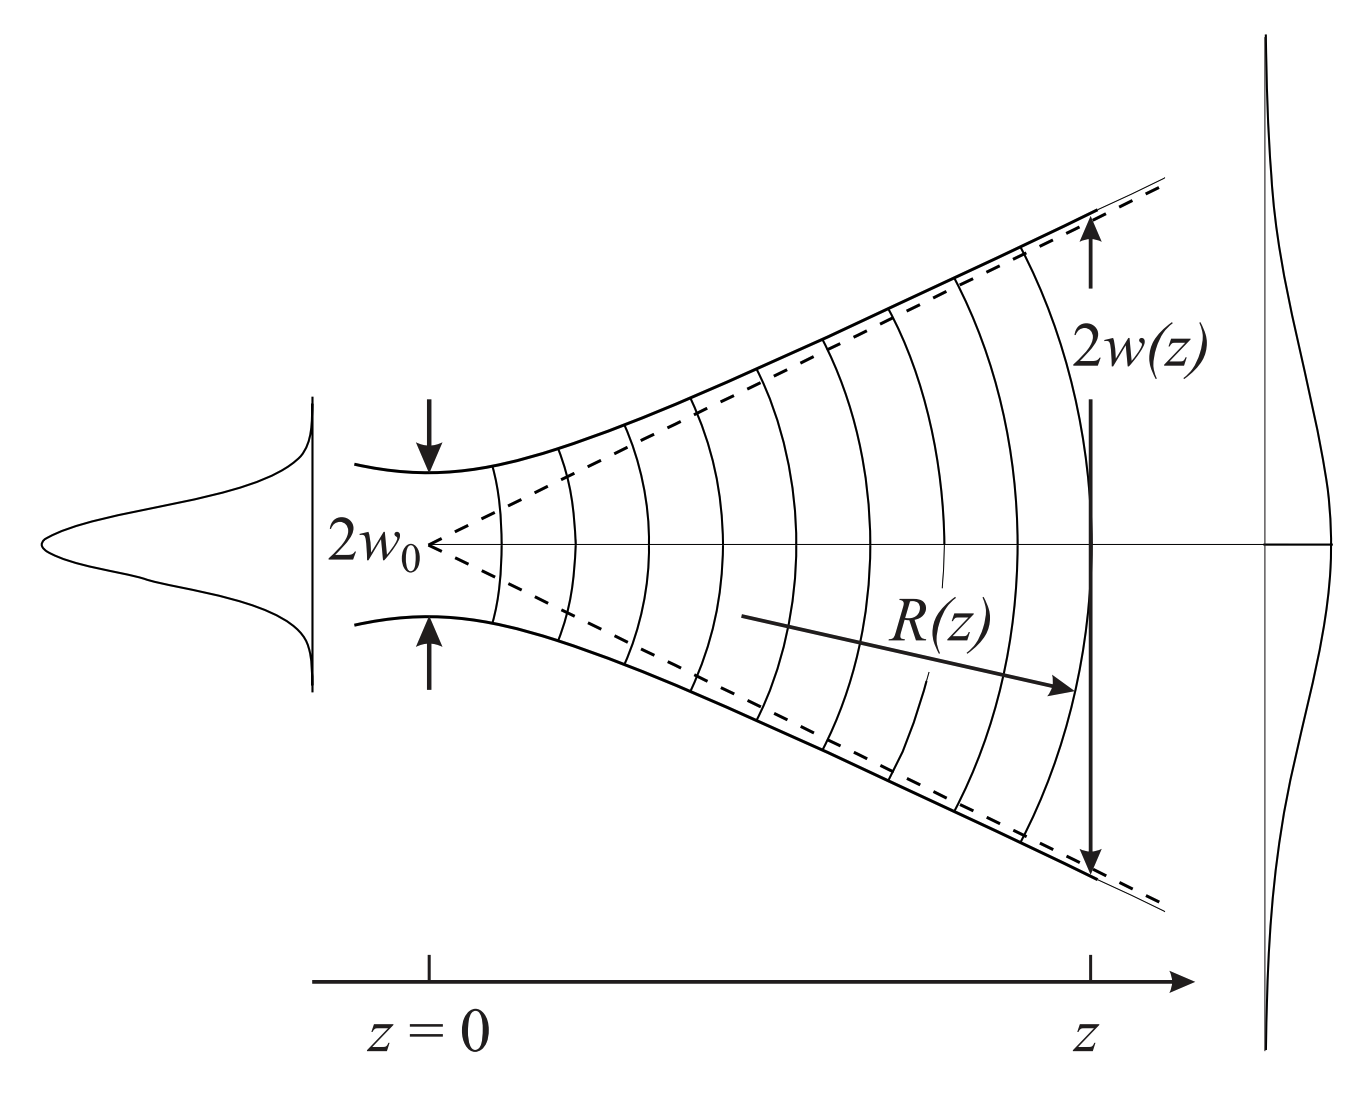
\includegraphics[width=8cm]{./img_chap4/img415a.png}
    \subcaption{Evolution of a Gaussian beam propagating along the z-axis\cite{riehle2006frequency}}{$w_0$ denotes a beam radius at beam weist, where $z=0$. $w(z)$ and $R(z)$ are the beam radius and curvature at $z$. Gouy phase is not shown in here.}\label{img:img415a}
  \end{minipage}\\
  \begin{minipage}{14cm}
    \centering        
    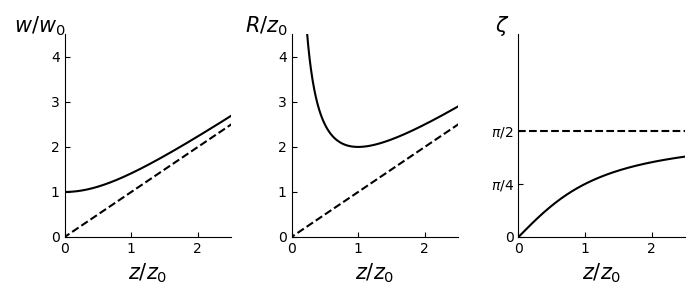
\includegraphics[width=14cm]{./img_chap4/img415.png}
    \subcaption{Beam prifile}{(left) Beam radius normalized by $w_0$ as a function of $z/z_0$, where $z_0$ is Rayleigh length. (Middle) Beam curvature normalized by $z_0$. (right) Gouy phase.}\label{img:img415}    
  \end{minipage}
  \caption{Gaussian beam.}
\end{figure}

As shown in Figure \ref{img:img415}, the beam profiles given by Eq.(\ref{eq:eq415_b},\ref{eq:eq415_c},\ref{eq:eq415_d}) are plotted as a function of $z$. In near-field ($z=0$), the beam can be regarded as the plane wave because the beam radius is smallest (beam waist), and the Gouy phase is 0. On the other hand, in far-field, the beam looks like a point source from far distant, and it is regarded as the spherical wave.
 % Theory
\bibliography{reference}
\bibliographystyle{unsrt}
\end{document}
